\documentclass[../../main.tex]{subfiles}
\begin{document}
\onlyinsubfile{
\setcounter{chapter}{3}
}
\notinsubfile{}
\chapter{Praktische opdrachten}\label{chap:H4}
De kennis van de vorige hoofdstukken kunnen we nu toepassen. Net als in het theoriedeel beperken we ons in dit hoofdstuk tot gebruik van re\"ele getallen. Alleen in de wiskunde verdieping gaan we verder. We zullen zien dat je met quantumcomputing heel andere dingen kunt doen dan met klassieke computers. Ook kun je de ontwikkelingen en de maatschappelijke implicaties verkennen.


\section{Protocol: BB84}\label{sec:poBB84}
\begin{wrapfigure}{o}{0.65\textwidth}
\centering
  \vskip-1cm
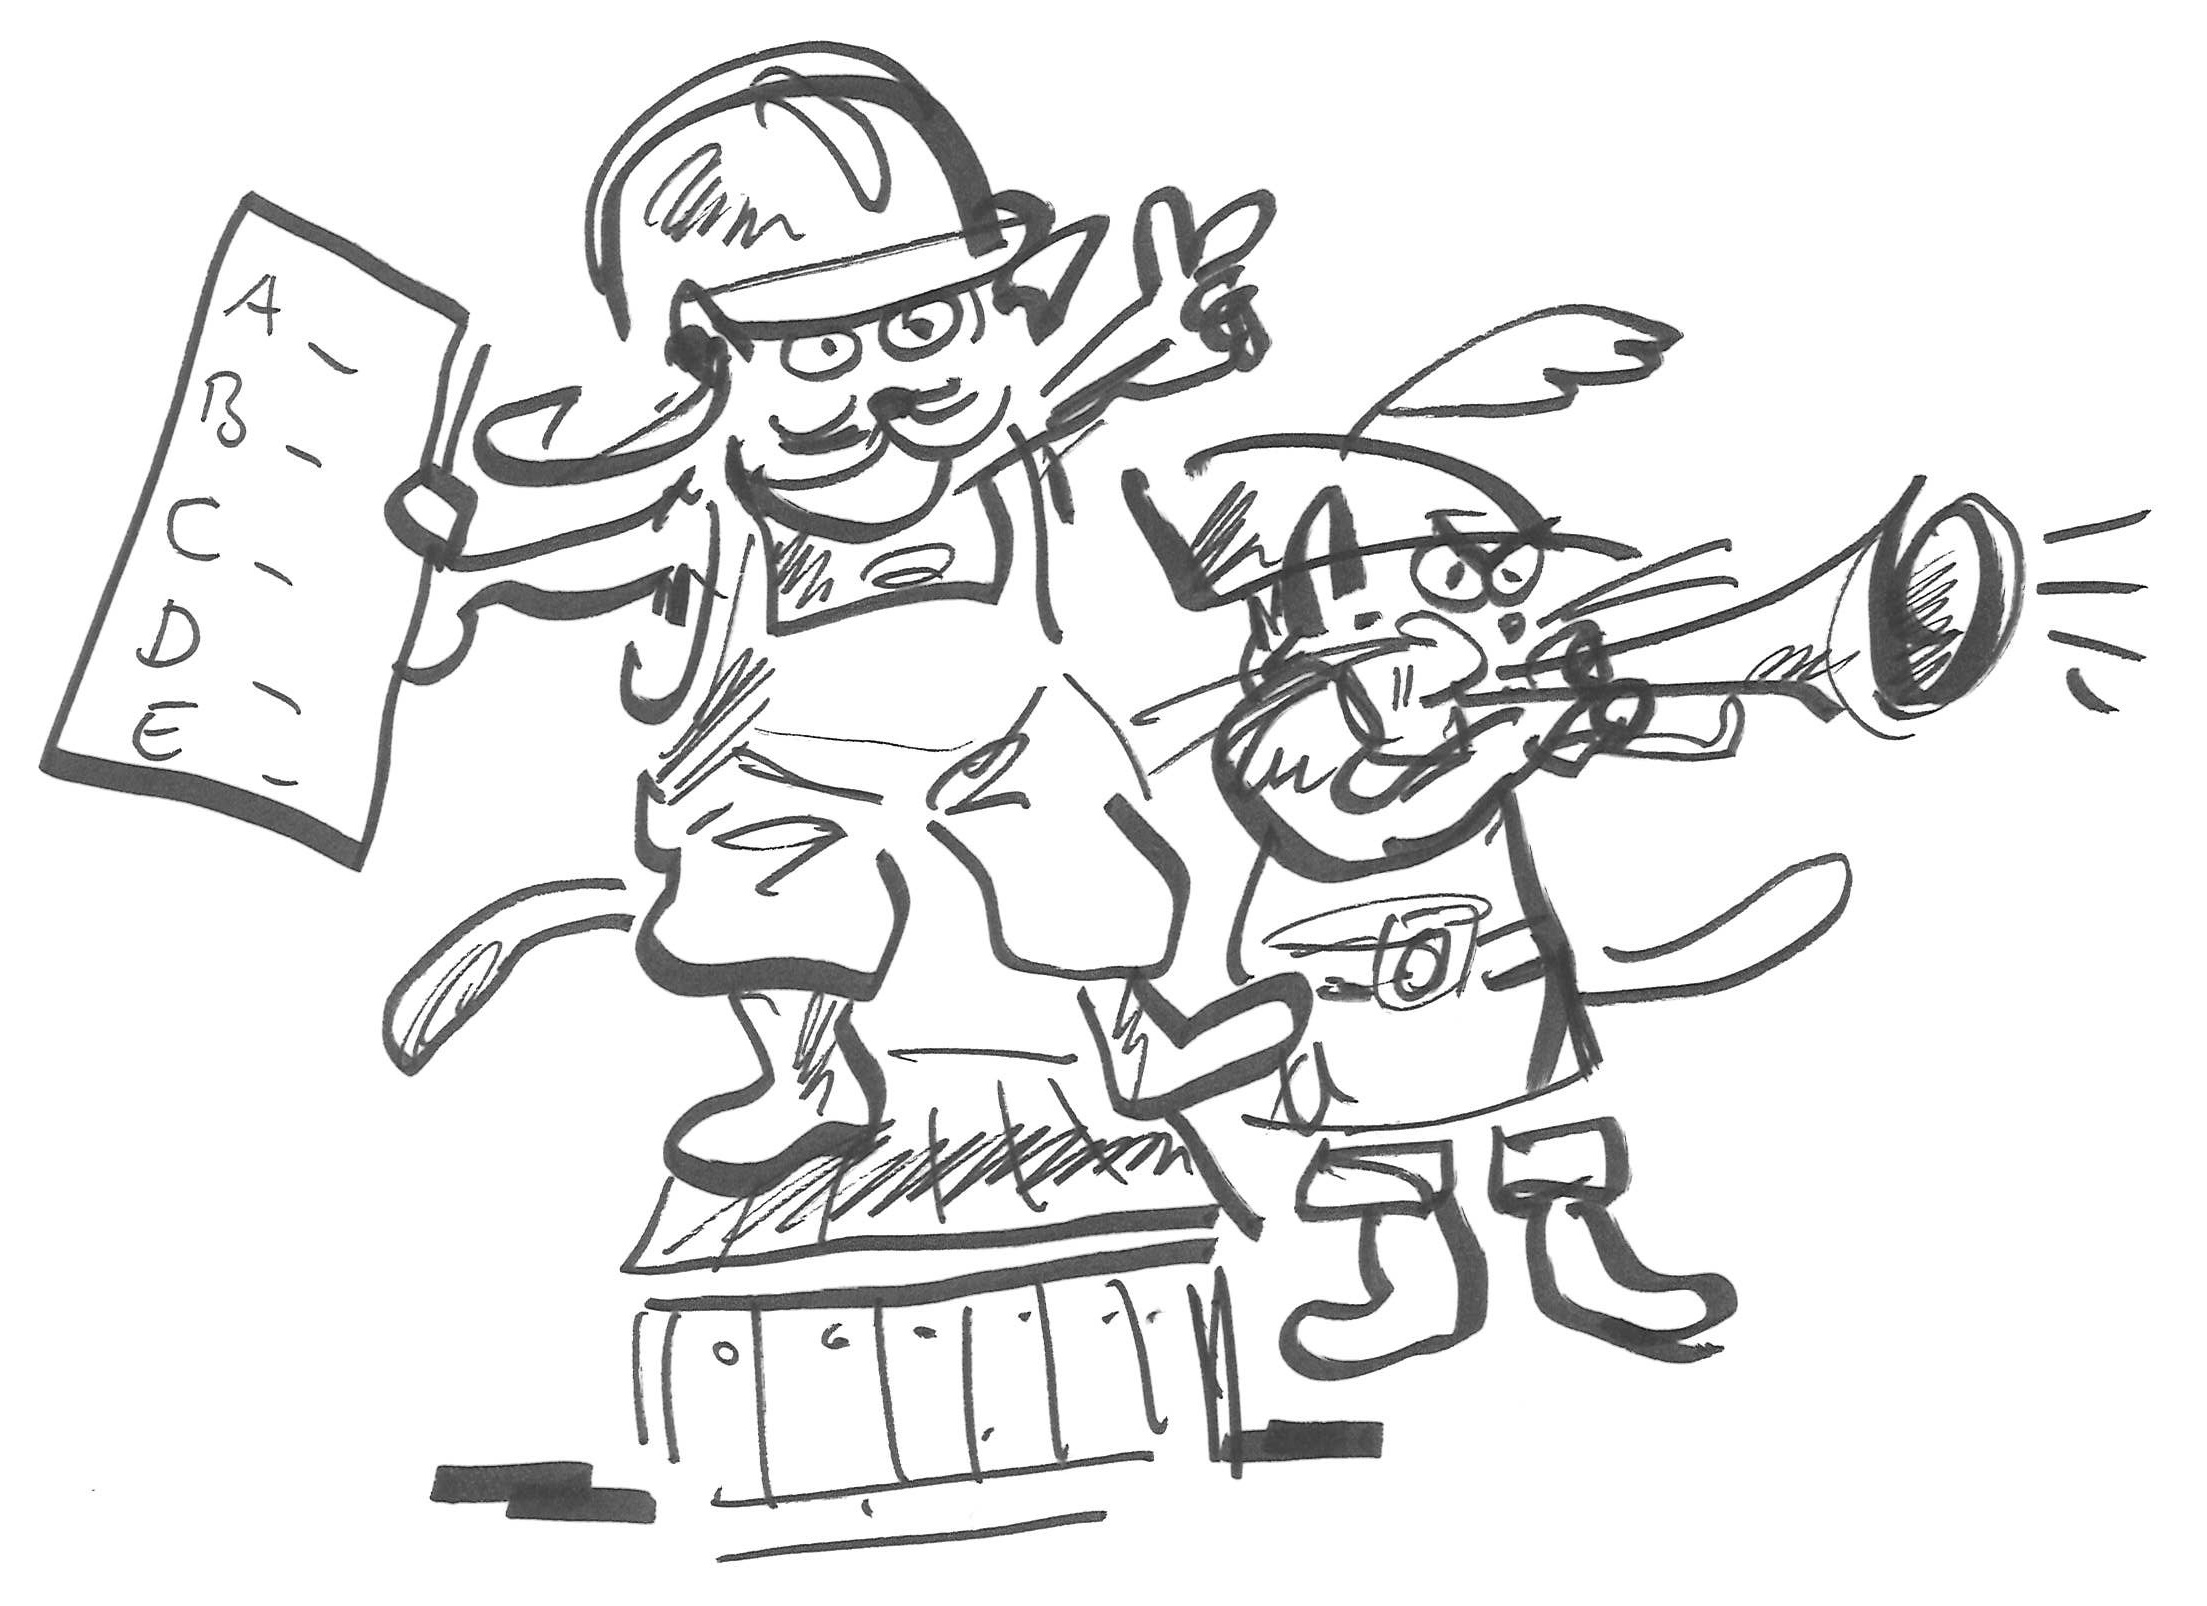
\includegraphics[width=0.65\textwidth]{./img/protocol.jpg}
\end{wrapfigure}
In hoofdstuk~\ref{chap:H1} hebben we met experimenten~\ref{sec:wbYoung1} en~\ref{sec:wbYoung2} de eigenschappen van gepolariseerd licht gebruikt om superpositie te introduceren. In hoofdstuk~\ref{chap:H2} en werkblad~\ref{sec:wbOVJV} 'Wat zie je' hebben we gezien hoe een waarnemer in een andere basis, andere co\"ordinaten aan dezelfde vector geeft. In dit werkblad werken we met die kennis een quantumencryptie-protocol uit. Dit protocol is in 1984 door Charles Bennet en Giles Brassard~\citep{BENNETT20147} gepresenteerd en geldt als eerste voorbeeld van onkraakbare code. Het staat bekend als BB84 en als quantum key distribution (QKD).


\begin{flushleft}
%\leavevmode
\begin{minipage}{.35\textwidth}
\def\ojfrangle{0}
\def\ojobangle{45}
\def\ojscale{.45}
\begin{tikzpicture}%
\begin{scope}[scale=\ojscale, rotate=\ojfrangle]
  \draw[thin,red!40] (-5,-5) grid (5,5);
  \draw[line width=.1pt ,black!30] ([shift=(-90:5)]0,0) arc (-90:180:5);
  \draw[-stealth,, red!40] (-0.1,0)--(5,0) node[below, red, xshift=10]{${\scriptstyle\ket{H}}$};
  \draw[-stealth, red!40] (0,-0.1)-- (0,5) node[left, red, yshift=0]{${\scriptstyle\ket{V}}$};
%  \draw[line width=.1pt ,black] ([shift=(0:5)]0,0) arc (0:90:5);
  \draw[thick, red, -stealth](0,0)--($cos(\ojobangle-\ojfrangle)*(5,0)$) node(x){};
  \draw[thick, red, -stealth](0,0)--($sin(\ojobangle-\ojfrangle)*(0,5)$) node(y){};
  \draw[thick, black!50, -stealth](0,0)--(\ojobangle-\ojfrangle:5) node (p){};
  \draw[loosely dashed] (x)--(p);
  \draw[loosely dashed] (y)--(p);
\end{scope}
\def\ojfrangle{-45}
\begin{scope}[scale=\ojscale,  rotate=\ojfrangle]
  \draw[thin,green!40!lightgray] (-5,-5) grid (5,5);
  \draw[-stealth, green!40!gray] (-0.1,0)--(5,0) node[right,  xshift=-3, yshift=-3]{${\scriptstyle\ket{-}}$};
  \draw[-stealth,green!40!gray] (0,-0.1)-- (0,5) node[above left,  xshift=13]{${\scriptstyle\ket{+}}$};
%  \draw[line width=.1pt ,black] ([shift=(0:5)]0,0) arc (0:90:5);
  \draw[thick, black, -stealth](0,0)--($cos(\ojobangle-\ojfrangle)*(5,0)$) node(x){};
  \draw[thick, black, -stealth](0,0)--($sin(\ojobangle-\ojfrangle)*(0,5)$) node(y){};
  \draw[thick, black!50, -stealth](0,0)--(\ojobangle-\ojfrangle:5) node (p){};
  \draw[ dotted] (x)--(p);
  \draw[ dotted] (y)--(p);
\end{scope}
\end{tikzpicture}
\end{minipage}%
\hfill
\begin{minipage}{.45\textwidth}
\[\begin{aligned}
\ket{+}&=\tfrac{1}{2}\sqrt{2}\ket{H}+\tfrac{1}{2}\sqrt{2}\ket{V}\\
\ket{-}&=\tfrac{1}{2}\sqrt{2}\ket{H}-\tfrac{1}{2}\sqrt{2}\ket{V}\\ 
\ket{H}&=\tfrac{1}{2}\sqrt{2}\ket{+}+\tfrac{1}{2}\sqrt{2}\ket{-}\\
\ket{V}&=\tfrac{1}{2}\sqrt{2}\ket{+}-\tfrac{1}{2}\sqrt{2}\ket{-}\\
\end{aligned}\]%subtiel veel minder whitespace
\captionof{figure}{In de standaardbasis (rood) wordt de zwarte vector met gelijke kans als $\ket{H}$ of $\ket{V}$ waargenomen. In de diagonale basis  (groen) wordt de vector met zekerheid als $\ket{+}$ waargenomen.}
\end{minipage}
%\caption{E\'en vector in standaardbasis (rood) en diagonale basis.}\label{fig:hvad}
%\end{figure}
\end{flushleft}

We gebruiken twee twee bases: de standaard basis en de diagonale basis. We weten hoe de Hadamard poort de standaardbasis op de diagonale basis afbeeldt \'en andersom. Het toestandsdiagram voor de \port{H}-poort en de vergelijkingen daarbij vind je bij fig.~\ref{fig:stateH}.
\marginpar{%
\[\begin{aligned}
\ket{0}\equiv\ket{H}\\
\ket{1}\equiv\ket{V}\\
\ket{+}\equiv\ket{D}\\
\ket{-}\equiv\ket{A}\\
\end{aligned}\]}

Fotonen zijn quantumdeeltjes die bij uitstek geschikt zijn voor het quantuminternet. Polarisatie blijft goed behouden over zeer lange lange afstanden, en fotonen reizen lekker snel, met de lichtsnelheid. Je kunt gepolariseerde fotonen versturen onder elke gewenste polarisatierichting. 

In deze communicatie zijn er twee partijen, Alice en Bob die op grote afstand van elkaar mogen staan. Ze gebruiken een quantumkanaal voor het verzenden van fotonen (glasvezelkabel), en een klassiek kanaal, een afluisterbare telefoon. Het quantumkanaal is \'e\'enrichting. Alice zendt een stroom fotonen naar Bob (\'e\'en richting), ieder foton in een door haar geprepareerde polarisatie. Ze noteert precies wat ze doet. Bij ontvangst meet Bob de fotonen via een polarisatiefilter dat hij willekeurig standaard of diagonaal zet. Ook hij houdt nauwkeurig bij wat hij doet. Ze verbreken de quantumverbinding en bellen elkaar. Via dit klassieke kanaal spreken ze met elkaar (bidirectioneel) het vervolg af. We werken deze stappen verder uit.

We weten  uit hoofstuk~\ref{chap:H1} dat als we een foton bijvoorbeeld verticaal polariseren en het vervolgens door een verticaal filter laten gaan, het foton met \textit{zekerheid} doorgelaten wordt, en dat het met \textit{zekerheid }geblokkeerd wordt als er een horizontaal filter volgt. Het gedrag is volledig voorspelbaar, \textit{deterministisch}. Als een verticaal gepolariseerd foton door een filter gaat dat onder \SI{45}{\degree} (of \SI{-45}{\degree}) staat, is er \SI{50}{\percent} kans dat het er doorheen gaat.

Alice wil uiteindelijk een boodschap als een reeks klassieke bits naar Bob sturen. Klassieke bits hebben de waarde $0_b$ of $1_b$. Ze houdt de volgende conventie aan:

\vspace*{12pt}
\begin{tabular}{c|c|cc|c|c}
bit & \multicolumn{1}{c|}{basis} & \multicolumn{2}{c|}{pol}\\\hline
logisch $0_b$& $\oplus$  &H &\rot{ 90}{$\updownarrow$}\\
logisch $0_b$& $\otimes$ &- &\rot{ 45}{$\updownarrow$}\\
logisch $1_b$& $\oplus$  &V &\rot{ 0}{$\updownarrow$}\\
logisch $1_b$& $\otimes$ &+ &\rot{-45}{$\updownarrow$}%
\end{tabular}
\vspace*{12pt}
%\nogdoen{NB in filmpje  delft diagonale basis basis juist andersom + =0 en -=1}

Alice heeft dus twee mogelijkheden om een $0_b$ te sturen en twee mogelijkheden voor een $1_b$. Als ze in de juiste basis worden waargenomen is het antwoord deterministisch. De informatie over haar eigen basiskeuze houdt Alice echter geheim. Alice heeft een string random bits gekozen en verzendt die ieder met een random basis.

Bob kan niet beter doen dan de binnenkomende fotonen meten volgens twee bases standaard (recht) en diagonaal. Bob kiest voor ieder foton een basis, en houdt nauwkeurig zowel de basiskeuze als het resultaat bij. Bob heeft geen idee of de basis waarmee hij meet dezelfde is als waarmee ze verzonden zijn. Ze verbreken daarna hun quantumverbinding. Hier onder een uitgewerkt voorbeeld;

\vspace*{12pt}
%\ifodd\thepage\else {\hspace*{-\fullmargin}}\fi
\begin{minipage}{\fullwidth}
{\footnotesize
\begin{tabular}{l|c|c|c|c|c|c|c|c|c|c|c|}
Alice' random bits&0&1&1&0&0&1&1&1&0&0\\\hline
Alice' basis      &$\otimes$&$\oplus$&$\otimes$&$\oplus$&$\oplus$&$\oplus$&$\otimes$&$\otimes$&$\oplus$&$\oplus$\\\hline
Alice verzendt    
       &\rot{ 45}{$\updownarrow$}
       &\rot{  0}{$\updownarrow$}
       &\rot{-45}{$\updownarrow$}
       &\rot{ 90}{$\updownarrow$}
       &\rot{ 90}{$\updownarrow$}
       &\rot{  0}{$\updownarrow$}
       &\rot{-45}{$\updownarrow$}
       &\rot{-45}{$\updownarrow$}
       &\rot{ 90}{$\updownarrow$}
       &\rot{ 90}{$\updownarrow$}\\ \hline
Bob's basis &$\oplus$&$\oplus$&$\otimes$&$\oplus$&$\otimes$&$\otimes$&$\otimes$&$\oplus$&$\otimes$&$\oplus$\\\hline 
Bob's meting&0&1&1&0&0&0&1&1&1&0
\end{tabular}}
\end{minipage}
\vspace*{12pt}

De rest van het protocol handelen ze af ze via de telefoon: Alice en Bob melden eerst hoeveel en welke bits bij Bob zijn overgekomen. Voor het gemak hier alle tien! Bob meldt Alice in welke basis hij heeft gemeten. Alleen als hun bases overeenkomen levert het zinnige informatie. De rest gooien ze weg.

Vraag: Hoeveel procent overeenkomst kun je verwachten als er een groot aantal bits verstuurd wordt?
\begin{antwoord}
 =\SI{50}{\percent}
\end{antwoord}

Ze weten nu over welke bits zij overeenstemming hebben zonder dat de data zelf is gecommuniceerd. Zij weten beiden bijvoorbeeld of een foton in de standaard basis horizontaal of verticaal was. Elk van de overgebleven fotonen bevat \'e\'en bit informatie uit Alice' random bit string.

\vspace*{12pt}
{\footnotesize
\begin{tabular}{c|c|c|c|c|c|c|c|c|c|c|c|}
Bob's basis & &$\oplus$&$\otimes$&$\oplus$& & &$\otimes$& & &$\oplus$\\\hline 
Bob's meting& &1&1&0& & &1& & &0
\end{tabular}
}

\paragraph{Afgeluisterd?}
Alice en Bob kunnen zijn afgeluisterd door Eve. Zij zou een foton door een filter kunnen leiden. Daarbij verliest het foton zijn eerdere informatie. Fotonen hebben geen geheugen. Ze kan het nooit meer terugzetten. Zij zou kunnen proberen een foton te versterken en dan een kopie uitlezen en het origineel doorsturen. Ook deze operatie is in tegenstrijd met de fundamenten van quantumtheorie \citep{wootters1982single}.
\iffalse
Gevolg is dat in geval ze afgeluisterd zijn \SI{50}{\percent} van de afgeluisterde fotonen de verkeerde informatie bevatten.
\fi
Alice en Bob testen of zij zijn afgeluisterd met een aantal goedgekeurde qubits (bijvoorbeeld een kwart van het totaal). Deze qubits kunnen ze verder niet gebruiken want ze zijn openbaar gemaakt.

\vspace*{12pt}
{\footnotesize
\begin{tabular}{c|c|c|c|c|c|c|c|c|c|c|}
Bob's publiceert  & & &1& & & &1& & & \\\hline 
Alice bevestigt:  & & &OK& & & &OK& & &
\end{tabular}
}
\vspace*{12pt}

Ze kunnen concluderen dat hun transmissie niet ernstig is afgeluisterd, anders konden ze opnieuw beginnen. De overgebleven bits kunnen worden gebruikt voor een \hrefqr[-1cm]{https://nl.wikipedia.org/wiki/One-time_pad}{one-time pad}. Dit is een sleutel voor de enig bewezen methode die onbreekbare vercijfering mogelijk maakt. Daarvoor moet de code nog wel aan extra eisen voldoen. Kijk op de bron welke vier eisen daar genoemd worden. 

Met het verkrijgen van de sleutel houdt het BB84 gedeelte van de encryptie op. De boodschap is een binaire reeks. De sleutel is precies even lang als de boodschap.
De \port{XOR}-poort is een logische poort (zie par.~\ref{sec:wbklassiek}) met de volgende waarheidstabel (zie fig.~\ref{fig:XOR}).

\begin{center}
\begin{minipage}[b]{.22\textwidth}
\begin{center}
\tikzstyle{branch}=[fill,shape=circle,minimum size=3pt,inner sep=0pt]
\begin{tikzpicture}[label distance=2mm]
    \node (x0) at (0,0) {$I_0$};
    \node (x1) at (0,-0.5) {$I_1$};
    \node[ xor gate US, draw, logic gate inputs=nn, anchor=input 1] at ($(x0)+(1,0)$) (Or1) {};
%    \node[not gate US, draw ] at ($(Or1.output)+(0.5,0)$) (Not2) {};
    \draw (x0) -- (Or1.input 1);
    \draw (x1) -| ([xshift=-0.5cm]Or1.input 2) -- (Or1.input 2);
    \draw (Or1.output) -- ([xshift=0.125cm]Or1.output) node[right] {$O$};
\end{tikzpicture}
\end{center}
\end{minipage}%
\hspace{0.25cm}
\begin{minipage}[b]{.22\textwidth}
{\scriptsize
\begin{tabular}{|l|l|l|}
\hline
$I_1$ & $I_2$ & O \\\hline
0    & 0  & 0 \\\hline
0    & 1  & 1 \\\hline
1    & 0  & 1 \\\hline
1    & 1  & 0 \\ \hline
\end{tabular}
}
\end{minipage}
\captionof{figure}{XOR-poort met waarheidstabel.\label{fig:XOR}}
\end{center}

Alice \port{XOR}-'t haar boodschap met de sleutel en zendt deze data over. 

Bob \port{XOR}-'t de boodschap met de sleutel. Wat is het resultaat?


Voorbeeld:

\vspace*{12pt}
%\ifodd\thepage\else {\hspace*{-\fullmargin}}\fi
\begin{minipage}{\fullwidth}
{\footnotesize
\begin{tabular}{l|c|c|c|c|c|c|c|c|c|c|c|}\hline
Alice' boodschap&1&0&0&1&0&1&0&0\\\hline
Alice' sleutel  &1&1&0&0&0&1&1&0\\\hline
Alice verzendt  &0&1&0&1&0&0&1&0\\\hline
\multicolumn{1}{c|}{\large \Phone}&\multicolumn{7}{c}{$\vdots$\hfill$\vdots$}\\\hline
Bob ontvangt    &0&1&0&1&0&0&1&0\\\hline
Bob's sleutel   &1&1&0&0&0&1&1&0\\\hline
Bob leest       &1&0&0&1&0&1&0&0\\\hline
\end{tabular}}
\end{minipage}
\vspace*{12pt}

\bigskip
Hoeveel fotonen moet Alice minimaal versturen als zij de boodschap "Heb je vanavond wat te doen?" wil overzenden zonder dat het afgeluisterd kan worden? Om een letterteken over te zenden zijn acht bits nodig. De zwakke quantumverbinding verliest \SI{20}{\percent} van de qubits.

\iffalse%-0-0-0-0-0-0-0
\begin{table}[h]
\leavevmode
\begin{tabular}{c|c|c|c|c|c|c|}
 basis &\rot{  0}{$\ominus$} 
       &\rot{  0}{$\ominus$}
       &\rot{ 45}{$\ominus$}
       &\rot{ 45}{$\ominus$}
       &\rot{  0}{$\ominus$} \\ \hline
 qubit &\rot{  0}{$\updownarrow$}
       &\rot{ 90}{$\updownarrow$}
       &\rot{ 45}{$\updownarrow$}
       &\rot{-45}{$\updownarrow$}
       &\rot{  0}{$\updownarrow$}\\ \hline
verzonden & 0 
          &$\ket{1}$ 
          &$\ket{-}$ 
          &$\ket{+}$ 
          &0
\end{tabular}
\end{table}


is de assen niet loodrecht zijn worden en enkele fotonen doorgelaten worden, dan zou je de stand van het eerste filter willen achterhalen. dat is echter onmogelijk. De fotonen die het tweede filter passeren hebben allemaal de ori\"entatie van het tweede filter. Fotonen hebben geen geheugen.
Kopi\"eren mag ook niet. \citep{wootters1982single}

De toestand van een foton kunnen we voorstellen als $\ket{\Psi}=\alpha\ket{\perp} +\beta\ket{\parallel}$ in co\
"ordinaten van de standaard basis.
We zouden ook een ander basis kunnen aannemen, de diagonale basis.
\[r_1=\mqty(1\\0), r_2=\mqty(0\\1), d_1=\frac{1}{\sqrt{2}}\mqty(1\\1), d_2=\frac{1}{\sqrt{2}}\mqty(1\\1)\]

\nogdoen{opm over geconjugeeerde basis, NB er is ook nog een complexe basis?}
Twee vectoren

We kunnen een foton prepareren in iedere polarisatietoestand. In ons model geven we de polarisatierichting van de filters aan met een rondje met een streep erdoor. De streep geeft aan in welke richting fotonen doorgelaten worden. Fotonen en hun polarisatierichting geven we met dubbele pijlen aan.
Aan de andere kant van de lijn staat Bob met een polaroid filter waarvan hij de ori\"entatie kan instellen. Als Bob een foton meet en het passeert het filter, dan met hij het als een bit 1. Als het er niet doorheen komt registreert hij een 0.
Klassieke bits dus. 

Als ongepolariseerd licht {\large\raisebox{0ex}{\rotatebox[origin=c]{30}{$\updownarrow$}}\hspace{-1em}}%
{\large\raisebox{.2ex}{\rotatebox[origin=c]{-35}{$\updownarrow$}}\hspace{-1.1em}}%
{\large\raisebox{-.1ex}{\rotatebox[origin=c]{-105}{$\updownarrow$}}}%
door een verticaal filter \rot{ 0}{$\ominus$} gaat, gaat het als verticaal gepolariseerd licht  $\updownarrow$ verder.
 
Als Alice \rot{-45}{$\updownarrow$} uitzendt heeeft Bob met een ze met een verticaal filter 50\% kans het foton om waar te nemen. Zie je de bewerking van de Hadamard poort terug?
c
Alice kan bij het verzenden kiezen uit twee bases van haar qubits. In de standaard basis ($\bigoplus$) $\updownarrow \leftrightarrow$ en in de diagonale basis ($\bigotimes$) $\updownarrow \leftrightarrow$. Ze kiest voor elk bit een random basis, maar houdt wel precies bij wat ze doet

Bijvoorbeeld

\begin{table}[h]
\leavevmode
\begin{tabular}{c|c|c|c|c|c|c|}
 basis &\rot{  0}{$\ominus$} 
       &\rot{  0}{$\ominus$}
       &\rot{ 45}{$\ominus$}
       &\rot{ 45}{$\ominus$}
       &\rot{  0}{$\ominus$} \\ \hline
 qubit &\rot{  0}{$\updownarrow$}
       &\rot{ 90}{$\updownarrow$}
       &\rot{ 45}{$\updownarrow$}
       &\rot{-45}{$\updownarrow$}
       &\rot{  0}{$\updownarrow$}\\ \hline
verzonden & 0 
          &$\ket{1}$ 
          &$\ket{-}$ 
          &$\ket{+}$ 
          &0
\end{tabular}
\end{table}

Aan de andere kant van de lijn meet Bob de qubits op. Hij heeft dezelfde twee bases ter beschikking. Hij weet niet met onder welke basis de bits verstuurd zijn.
Als hij dezelfde basis meet als waarin ze verstuurd zijn, meet hij het bit correct \nogdoen{(is dat zo orientatie over afstand)}.
Er is 50\% kans dat hij de verkeerde basis kiest. Ook dan heeft  heeft hij 50\% kans dat het bit goed gemeten wordt.

In 75\% van de gevallen zullen Alice' en Bob's metingen dus overeenkomen.
Ook Bob houdt nauwkeurig de gemeten waarde van de qubits bij en ook in welke basis hij gemeten heeft.

Bob meet bijvoorbeeld als volgt:
\begin{table}[h]
\leavevmode
\begin{tabular}{c|c|c|c|c|c|c|}
 basis &\rot{  0}{$\ominus$} 
       &\cellcolor{red!50}\rot{  0}{$\ominus$}
       &\rot{ 45}{$\ominus$}
       &\rot{ 45}{$\ominus$}
       &\rot{  0}{$\ominus$} \\ \hline
 qubit &\rot{  0}{$\updownarrow$}
       &\cellcolor{red!50}\rot{ 90}{$\updownarrow$}
       &\rot{-45}{$\updownarrow$}
       &\rot{ 45}{$\updownarrow$}
       &\rot{  0}{$\updownarrow$}\\ \hline
verzonden & 0 
          &\cellcolor{red!50}$\ket{1}$ 
          &$\ket{1}$ 
          &0 
          &1 
\end{tabular}
\end{table}


Alice en Bob bellen elkaar nu op met een gewone telefoon. 
Ze delen en vergelijken de stand van hun filters (bases, maar houden de waarden van hun verzonden en gemeten bits geheim.

Ze gooien de gegevens weg als hun bases niet overeenkomen. Dat is de helft van de data.We houden 2N gegevens over.

Van die data weten zij


NB geen verstrengeling nodig, gebaseerd op no-cloning

4N data


eve

ruis

$\updownarrow \leftrightarrow$

$\nearrow \searrow\uparrow\downarrow$

$\bigoplus\bigotimes \ominus \oslash $

$\leftrightarrow$
\rotatebox[origin=c]{45}{$\leftrightarrow$}
\rotatebox[origin=c]{-45}{$\leftrightarrow$}

$\ominus$ \rotatebox[origin=c]{90}{$\ominus$}
$\oslash$ \rotatebox[origin=c]{90}{$\oslash$}

\rot{  0}{$\updownarrow$}
\rot{ 90}{$\updownarrow$}
\rot{ 45}{$\updownarrow$}
\rot{-45}{$\updownarrow$}

\rot{  0}{$\ominus$}
\rot{ 90}{$\ominus$}
\rot{ 45}{$\ominus$}
\rot{-45}{$\ominus$}


\rot{ 0}{$\oslash$}
\rot{90}{$\oslash$}

%$\varobar\bigoslash$

open access:
\cite{BENNETT20147} Dit hele issue is open access
kunnen niet tussentijds versterkt worden, niet geschikt als digitale handtekening, versleutelde mail(?), of een oplossing bieden in een juridisch dispuut 
\cite{wootters1982single}

\marginnote{trapdoor function valluik functie: een functie die de ene klant op makkelijk, maar de andere kant op moeijk is.
(bijvoorbeeld kwadrateren is makkelijker dan worteltrekken)
one-time pad sleutel}

Hoe doen we dat in een computerspelletje
computerspelletje:
Begin bij het einde:\\
Welke boodschap wil je sturen?\\
-Zullen we een biertje drinken?\\
-Heb je vanavond wat te doen?\\
-eigen tekst ...\\

Hoeveel bits heb je minimaal nodig om deze boodschap met BB84 over te zenden (NB elke letter bestaat uit 8 bits)? 30 letters=240b dus: N=240

4N=960bits
Alice genereert een string van 960 random bits en een string van 
960 basiskeuzen (D/R)
Horizontaal \rot{  0}{$\updownarrow$} en \rot{ 45}{$\updownarrow$} stellen een 0 voor, \rot{ 90}{$\updownarrow$} en \rot{-45}{$\updownarrow$} een 1.

Bob besluit voor ieder foton zelf in welke basis hij meet. Hij interpreteert de resultaten consequent als binair 0 of 1. Ook hij houd nquwkeurig bij wat zijn metingen zijn en welke stand zijn filter daarbij is.

Bob en Alice verbreken hun quantumverbinding en pakken de telefoon. \nogdoen{de telefoon kan afeluisteerd worden, maar kan geen boodschappen tussenvoegen of veranderen}.

Zij stellen vast welke fotonen zijn \"uberhaupt ontvangen zijn en welke daarvan onder dezelfde basis zijn gemeten. 

Elk foton staat vor \'e\'en bit random informatie (bijvoorbeeld wanneer een rechtop foton verticaal of horizontaal was). Deze informatie is alleen aan Alice en Bob bekend.
\nogdoen{test for evesdropping, ongeveer een derde van de correcte bits}


Bob's basiskeuze is random en zal naar verwachting voor de helft van de gevallen overeenkomen met die van Alice. De rest van de data is waardeloos maar levert wel in de helft van de gevallen de juiste informatie op.

Bob's foton detectors zijn niet perfect. Sommige fotonen zal hij niet registreren.

----
\hrefqr{https://www.youtube.com/watch?v=lVXJgn3fDkg&ab_channel=QuTechAcademy}{filmpje Tim Coopmans} geeft een goede uitleg, maar op basis van Bloch bol.
Verander op basis van XY vlak (loodrecht en 45 graden bases 
Niet in het filmpje hoe het aantal bits van 4N naar N gaat.
\fi%-0-0-0-0-0-0

\section{Eerlijk quantummuntje}
Een andere toepassing van het BB84 protocol is deze quantumtoss. Alice en Bob hebben ruzie. Ze willen elkaar even niet zien. Wie mag met de auto weg? Ze bellen elkaar op. Bob ziet het al voor zich:
Alice daagt uit tot een kop of munt spelletje over de telefoon. Zij vraagt kop of munt? Wat ik ook kies, zeg zegt gewoon wat haar uit komt. Ze liegt. Dat deed ze vorige keer ook. Ze vertrouwen elkaar even niet.

(De telefoon gaat). Bob: Ja?\\
(Alice): Alice hier. Kan ik de auto vanmiddag ...\\
(Bob): Nee\\
(Alice): Het is ook mijn auto! Laten we er om loten?\\
(Bob): Ok?\\
(Alice): Ik gooi een muntje op. Kop of munt?\\
(Bob): Ja zeg, net als vorige keer zeker.\\
(Alice): Vertrouw je me niet?\\
(Bob): Nee!\\
(Alice): Tsss\\
(Bob zucht): Ok, we doen het zo. We gebruiken een quantumbasis 'R' of 'D' in plaats van kop of munt.\\
Alice: Hmmm, ok dan.\\
 
\iffalse
volgende filmpje is helaas te ingewikkeld. \hrefqr{https://ocw.tudelft.nl/course-lectures/8-5-2-coin-flipping-phone/}{filmpje TuD}
\fi
Alice kiest een reeks random bits (bv \SI{1}{\kilo\bit}) en \'e\'en willekeurige basis, bijvoorbeeld "R". Ze kiest een codering ($H=1_b$, $V=0_b$).

Alice verstuurt haar reeks van gepolariseerde fotonen.

Bob kiest voor ieder foton dat hij ontvangt een basis, onafhankelijk en willekeurig voor elk foton.

Niet alle fotonen komen over, er zijn gaten in de ontvangstabel.

Na ontvangst belt hij Alice en zegt welke basis zij heeft gekozen.

Als hij goed geraden heeft wint hij, anders verliest hij.

Alice meldt of Bob gewonnen of verloren heeft en zendt ter controle nogmaals de reeks random bits waar zij mee begon.

Bob controleert de reeks tegen zijn tabellen. Er moet een perfecte match zijn met de kolommen in Alice' basis, en een random relatie bij de andere kolommen. 
\iffalse%-9-9-9-9-------------------------------------------

\vspace*{12pt}
%\ifodd\thepage\else {\hspace*{-\fullmargin}}\fi
\begin{minipage}{\fullwidth}
{\footnotesize
\begin{tabular}{l|c|c|c|c|c|c|c|c|c|c|c|}
Alice' random bits&0&1&1&0&0&1&1&1&0&0\\\hline
Alice' basis  &\multicolumn{7}{c}{R}\\\hline
Alice verzendt    
       &\rot{ 90}{$\updownarrow$}
       &\rot{  0}{$\updownarrow$}
       &\rot{  0}{$\updownarrow$}
       &\rot{ 90}{$\updownarrow$}
       &\rot{ 90}{$\updownarrow$}
       &\rot{  0}{$\updownarrow$}
       &\rot{  0}{$\updownarrow$}
       &\rot{  0}{$\updownarrow$}
       &\rot{ 90}{$\updownarrow$}
       &\rot{ 90}{$\updownarrow$}\\ \hline
Bob's basis    &R&R&D&R&D&D&D&R&D&R\\\hline 
Bob's "R" tabel&0&1& &0& & & &1& &0\\\hline 
Bob's "D" tabel& & &1& &1&0&0& &0& \\\hline 
\multicolumn{1}{c|}{\large \Phone}&\multicolumn{7}{c}{}\\\hline
Bob's gok&\multicolumn{7}{c}{R?}\\\hline
Alice' antwoord&\multicolumn{7}{c}{Haha, fout!}\\\hline
Bob's gok&\multicolumn{7}{c}{SStuur toch effe jouw reeks}\\\hline
Alice stuurt origineel&0&1&1&0&0&1&1&1&0&0\\\hline
Bob's "R" tabel&0&1& &0& & & &1& &0\\\hline 
Bob's "D" tabel& & &1& &1&0&0& &0& \\\hline 
\end{tabular}}
\end{minipage}

Bob: Alice! Hier met die auto!\vspace*{12pt}

Dit lijkt een waterdicht systeem, maar Alice is ook slim. Zij heeft Einsteins artikel gelezen en Hoofdstuk vier ...

Samenvatting in \hrefqr{https://math.stackexchange.com/questions/239202/how-to-perform-a-fair-coin-toss-experiment-over-phone}{stackexchange}
\begin{enumerate}
\item Alice chooses two large prime numbers $p$ and $q$, with the property $p\equiv 3 mod 4$ and $q \equiv 3mod4$. She computes the number $n=pq$ and reads it to Bob over the phone. She keeps the numbers p and q secret.

\item Bob chooses a random integer $x$ between $1$ and $n$. He computes the square $a= x2 mod n$ and reads it to Alice over the phone. He keeps the number $x$ secret.

\item Since Alice knows the factorization of $n$, she can compute the square roots of a modulo $n$. There are four such square roots, let's say $x$ and $n-x$ and $x^{\prime}$ and $n-x^{\prime}$. Alice can compute them all, but she does not know which number Bob has chosen. Alice chooses one of these square roots and reads it to Bob over the phone.

\item Bob compares the number read to him over the phone to the number that he chose. If Alice communicated the number $x$ or $n-x$, he says to Alice "you win, but you must now tell me the factors $p$ and $q$". Then Alice reads the factors $p$ and $q$ to him over the phone, and Bob can check that they are both prime numbers and that $n=pq$. The game is over, and Alice has won.

\item If Alice communicated the number $x^{\prime}$ or $n-x^{\prime}$, Bob can use this information and the fact that he knows the other square root, namely $x$, to find the factors of $n$. He does this, and he says to Alice "you lose, here are your factors". The game is over, and Bob has won.
\end{enumerate}
\fi%-9-9-9-9------------------------------------------



\clearpage
\section{Protocol: Superdense coding}\label{sec:poSuperdense}

In deze opdracht ga je onderzoeken hoe je door gebruik te maken van qubits, boodschappen kunt communiceren. Je kunt twee klassieke bits vervangen door \'e\'en qubit. Dit heet \textit{superdense coding}. De opdracht bestaat uit drie delen. Eerst zullen we superdense coding bekijken en is er een aantal opgaven. Daarna ga je zelf een klein quantum communicatiesysteem ontwerpen en programmeer je dit systeem in Quantum Inspire. Aan het eind van de opdracht presenteer je je bevindingen.

\subsection*{Communiceren op een eiland}
Alice woont alleen op een eiland. Ze heeft met niemand contact, behalve met Bob, die op het vasteland woont en die ze berichten kan sturen als er dingen op het eiland misgaan. In eerste instantie kan Alice alleen klassieke bits met Bob uitwisselen. Ze hebben de volgende codering afgesproken:\\
\\
00 – SOS!\\
01 – Nieuw materiaal voor huis nodig\\
10 – Er is droogte/geen water op het eiland\\
11 – Er is geen voedsel op het eiland\\
\\
Alice verstuurt de bits altijd \'{e}\'{e}n voor \'{e}\'{e}n naar Bob; eerst het bit dat achteraan staat en dan het voorste bit. Ze begint altijd met beide bits in 0 (00). Wanneer ze nieuw materiaal nodig heeft voor haar huisje, zal ze dus haar achterste bit eerst moeten flippen alvorens haar boodschap naar Bob te sturen. En als Alice voedsel nodig heeft, moet ze beide bits flippen. Alleen als Bob een volledige code ontvangt, kan hij Alice helpen. Immers, als Bob enkel een 0 ontvangt en het tweede bit ontbreekt, kan dat ofwel 'SOS', ofwel 'water nodig' betekenen. Om een boodschap over te laten komen, \emph{moet} Alice dus twee bits versturen.

Dan hoort Bob over qubits en verstrengeling van Julia. Alice en Bob besluiten daartoe om over te stappen op quantumcommunicatie. Om dit mogelijk te maken, delen ze twee volledig verstrengelde qubits in een van de Bell-toestanden. De Bell-toestanden zijn:

G: $\tfrac{1}{\sqrt{2}}\ket{00}+\tfrac{1}{\sqrt{2}}\ket{11}$\\
H: $\tfrac{1}{\sqrt{2}}\ket{00}-\tfrac{1}{\sqrt{2}}\ket{11}$\\
J: $\tfrac{1}{\sqrt{2}}\ket{10}+\tfrac{1}{\sqrt{2}}\ket{01}$\\
K: $\tfrac{1}{\sqrt{2}}\ket{10}-\tfrac{1}{\sqrt{2}}\ket{01}$\\

Alice en Bob delen de eerste Bell toestand G: $\frac{\ket{\textcolor{red}{0}\textcolor{blue}{0}}+\ket{\textcolor{red}{1}\textcolor{blue}{1}}}{\sqrt{2}}$. Alice krijgt de eerste (\textcolor{red}{rode}) qubit, Bob houdt de tweede (\textcolor{blue}{blauwe}) qubit. Door poorten op haar qubit toe te passen, kan Alice van toestand G in een van de andere Bell-toestanden komen. Als Alice bijvoorbeeld een X-poort op haar qubit toepast, delen Bob en zij toestand J, zonder dat Bob iets met zijn qubit heeft gedaan. En om toestand H te krijgen, hoeft Alice alleen een Z-poort op haar qubit toe te passen. Alice en Bob zouden nu hun vier verschillende boodschappen aan de Bell-toestanden kunnen hangen (maakt Alice de toestand G, dan betekent dat `SOS', etc.) Door haar qubit te roteren, kan Alice elke Bell-toestand maken die ze wil. Vervolgens stuurt Alice haar qubit naar Bob. Bob meet het verstrengelde paar en weet welke boodschap Alice wilde overbrengen. Het bijzondere hieraan is dat Alice in dit geval slechts \'{e}\'{e}n qubit hoeft te versturen om dezelfde boodschap over te brengen waarvoor ze met klassieke communicatie \emph{twee} bits nodig had. Vandaar de naam voor dit protocol!

\begin{antwoord}
a) toestanden zijn niet te isoleren door ontbinding $\alpha\ket{0}+\beta\ket{1}$\\
\end{antwoord}
\begin{opdrachtlang}
\begin{enumerate}
\item Laat zien dat toestand G inderdaad verstrengeld is.
\item Teken het schema om van twee losse qubits in de toestand $\ket{0}$ in verstrengelde toestand (G) te komen.
\item Welke quantumpoort(en) moet Alice op haar qubit toepassen om de toestand K te krijgen?
\item Kan \'e\'en qubit nu twee bits aan informatie opslaan?
\item Zou dit schema ook werken als Alice en Bob twee qubits hadden die niet verstrengeld waren? Waarom wel/niet?
\item In het teleportatieprotocol van hoofdstuk drie heb je gezien dat er een klassiek kanaal nodig is om een quantumtoestand (quantumboodschap) over te brengen. Wat voor kanaal (klassiek/quantum) wordt er bij superdense coding gebruikt en wat voor boodschap (klassiek/quantum)?
\item Bob zou de qubits kunnen meten in een speciale Bell-basis, maar hij besluit de qubits te meten in de $\ket{0}$/$\ket{1}$-basis. Hiertoe moet hij de verstrengelde toestand terugbrengen tot twee losse qubits. Het protocol om dit te doen is precies tegenovergesteld aan het protocol om twee qubits te verstrengelen. Teken het schema en laat zien dat Bob op deze manier inderdaad de qubits kan decoderen en de boodschap kan ontcijferen. Welke boodschap hoort dus bij welke Bell-toestand?
\end{enumerate}
\end{opdrachtlang}
\subsection*{Uitgebreidere communicatie}
Alice vindt haar communicatiemogelijkheden met Bob maar gelimiteerd. Ze wil graag meer boodschappen kunnen overbrengen. Ze stelt daarom aan Bob voor om drie verstrengelde qubits te delen (dit heet een GHZ toestand):

\[\begin{aligned}
M: \alpha\ket{000}+\beta\ket{111}
\end{aligned}\]

Hier kan Alice 8 boodschappen mee versturen ($2^3=8$). Bedenk nu zelf een schema waarbij Alice deze acht boodschappen kan versturen. Denk hierbij aan het volgende:
\begin{itemize}
\item Schrijf de acht GHZ toestanden uit die gemaakt kunnen worden.
\item Teken het schema om drie qubits die beginnen in de toestand $\ket{0}$ in de GHZ-toestand $M$ te krijgen.
\item Teken het schema om drie qubits die beginnen in de toestand $\ket{0}$ in een willekeurige andere GHZ-toestand te krijgen.
\item Hoeveel van deze GHZ-toestanden kan Alice maken als ze zelf de eerste qubit heeft en Bob de laatste twee? 
\item Hoeveel van deze GHZ-toestanden kan Alice maken als ze zelf de eerste twee qubits heeft en Bob de laatste?
\item Als Alice zelf twee qubits heeft, welke poorten moet zij dan toepassen op toestand M om naar de andere GHZ toestanden te komen?
\item Beschrijf hoe het protocol werkt als Alice twee qubits heeft en Bob \'{e}\'{e}n. Teken het schema, inclusief het maken van de GHZ-toestand en het decoderen en uitlezen ervan door Bob.
\end{itemize}

\begin{opdrachtlang}
We gaan nu kijken of alle voorspellingen kloppen door het protocol te bouwen op Quantum Inspire. Open hiertoe Quantum Inspire en voer de volgende opdrachten uit:

\begin{itemize}
\item Bouw het protocol waarbij Alice en Bob een Bell-toestand delen (je kunt hiervoor zelf kiezen welke van de twee quantumchips je gebruikt). Bouw het hele protocol, begin met twee qubits in $\ket{0}$, maak hiervan een verstrengeld paar, verzin welke boodschap je wilt versturen, voer Alice's handelingen uit en decodeer de toestand alvorens je deze meet. Doe dit voor alle vier de boodschappen. Zijn de uitkomsten zoals je verwachtte?
\item Bouw het protocol waarbij Alice en Bob een GHZ-toe\-stand delen, waarbij Alice begint met 2 qubits en Bob met 1 qubit. Je kunt dus 8 boodschappen versturen (je moet hiervoor de quantumchip met 5 qubits gebruiken). Bouw het hele protocol; verstrengel de drie qubits, codeer een boodschap, decodeer de boodschap en meet de qubits. Doe dit voor alle acht de boodschappen. Zijn de uitkomsten zoals je verwachtte?
\item Bouw een protocol waarbij Alice en Bob twee Bell-toe\-standen delen. Van beide toestanden heeft Alice de eerste qubit en Bob de tweede qubit (je moet hiervoor de quantumchip met 5 qubits gebruiken). Bouw opnieuw het hele protocol, van het verstrengelen van beide paren en het coderen van de boodschap tot het decoderen van de boodschap en het meten van de qubits. Hoeveel boodschappen kan Alice nu versturen en hoeveel qubits heeft ze naar Bob gestuurd?

\item Vind je het effici\"{e}nter als Alice en Bob een GHZ-toestand delen, of twee verstrengelde paren?
\end{itemize}
\end{opdrachtlang}
%\begin{antwoord}
%\end{antwoord}

\clearpage
\section{Quantum en maatschappij} \label{sec:poquantumenmaatschappij}

\begin{quote}
Quantumtechnologie is een sleuteltechnologie die radicaal nieuwe producten en diensten mogelijk maakt. Quantumcomputers, quantumsimulators, quantumnetwerken en quantumsensoren kunnen straks dingen die 'klassieke' apparaten niet kunnen. [...] We staan daarmee aan het begin van een technologierevolutie die verwacht wordt een grote bijdrage te leveren aan het oplossen van maatschappelijke uitdagingen op het gebied van bijvoorbeeld energie, voedsel en zorg. Nederland doet mee in de wetenschappelijke en technologische voorhoede van de ontwikkelingen en wereldwijd wordt er door overheden en bedrijven fors geïnvesteerd in quantumonderzoek en -innovatie.
\end{quote}

Zo begint het rapport van de Nationale Agenda Quantumtechnologie, opgesteld in september 2019 in opdracht van het  Ministerie van Economische Zaken en Klimaat. Het duidelijk: de quantumcomputer komt er aan.
In een opdracht over de maatschappelijke impact van deze tweede quantumgolf (de eerste vond plaats in het begin van de twintigste eeuw) mag een gedachtewisseling over deze ontwikkelingen niet ontbreken. In opdracht \ref{opd:lang} lezen we de Nationale Agenda door. 
\begin{opdrachtlang}\label{opd:lang}%
Voor deze opdracht moet je gebruik maken van internet. Je doet de opdracht  met zijn  twee\"en. 
\begin{enumerate}
\item Download de \hrefqr{https://quantumdelta.nl/TUQ/wp-content/uploads/2020/03/NAQT-2019-NL.pdf}{Nationale Agenda} 

\item De Nationale Agenda noemt behalve de quantumcomputer nog drie andere  toepassingen van quantumtechnologie in bovenstaand citaat. Zoek in de brochure op wat deze technologie\"en inhouden.
\end{enumerate}
In \textbf{hoofdstuk~1} vind je een overzicht van de inhoud van de brochure.
\begin{enumerate}[resume]
\item Geef in trefwoorden de inhoud van de  brochure van de verschillende hoofdstukken.
\end{enumerate}
\textbf{Hoofdstuk~2} geeft de vier belangrijkste toepassingsgebieden die ook voor het Europese Quantum Flagship  van belang zijn.  Bij de beschrijving van deze  vier toepassingsgebieden worden belangrijke details vermeld.
\begin{enumerate}[resume]
\item Wat is het verschil tussen universele quantumcomputers en quantumsimulatoren?
\item Wat is een hybride quantumsimulator?
\item Wat zijn de voordelen van quantumcommunicatie op wereldschaal?
\item Welke domeinen kunnen profiteren van quantumsensing?
\end{enumerate}
\textbf{Hoofdstuk~3} gaat over de relatie tussen quantumtechnologie en maatschappij. In figuur~7 van de module is die relatie in kaart gebracht. 
\begin{enumerate}[resume]
\item Geef aan op welke  maatschappelijke terreinen quantumtechnologie  een rol gaat spelen. Geef voor elk terrein een voorbeeld van een toepassing.
\end{enumerate}
\textbf{Hoofdstuk~4} brengt de positie van Nederland op quantumgebied in kaart. Daarbij wordt ook aandacht gegeven aan Nederlandse kennisinstellingen en universiteiten.
\begin{enumerate}[resume]
\item Geef bij figuur~7 voor elk van de maatschappelijke terreinen één universiteit/kennisinstelling aan die op dat terrein actief is. 
\end{enumerate}
\textbf{Hoofdstuk~5} beschrijft vier lijnen waarop moet worden geacteerd en drie katalysator-programma's.
\begin{enumerate}[resume]
\item Noem de vier lijnen en beschrijf de drie programma's.
\end{enumerate}
\textbf{Hoofdstuk~6} gaat over de Nederlandse overheid.
\begin{enumerate}[resume]
\item Geef met twee werkwoorden aan wat de Nederlandse overheid volgens de brochure moet doen.
\end{enumerate}
\end{opdrachtlang}
  
\subsection*{Wat gaat de gemiddelde burger merken van de quantumcomputer?}  
De quantumcomputer zal de gewone PC niet gaan vervangen. De digitalisering die overal om ons heen plaats vindt gaat gewoon door. En daarbij wordt gebruik gemaakt van bits en niet van qubits. Niettemin is uit het voorgaande ook op te maken dat de wereld om ons heen gaat veranderen door de komst van de quantumcomputer. Er wordt zelfs gesproken van een nieuwe technologische revolutie. In opgave \ref{opd:overzicht} doe je een poging om in kaart te brengen hoe die revolutie er uit gaat zien.



\begin{opdracht}\label{opd:overzicht}
Maak aan de hand van de teksten en interviews in het voorgaande een overzicht van alle mogelijke ontwikkelingen op het gebied van de quantumtechnologie.
\begin{enumerate}
\item Begin met de Nationale Agenda, hoofdstuk~3, figuur~7. Denk na over de wijze waarop je de ontwikkelingen in kaart brengt. Maak eventueel gebruik van een matrix om overzicht te krijgen.
\item Loop de andere bronnen langs om te kijken of er nog waardevolle aanvullingen zijn. 
\end{enumerate}
\end{opdracht}

De Nationale Agenda voor Quantumtechnologie is zelfverzekerd; de quantumcomputer gaat er komen. Dat verwacht je ook  van zo'n rapport. Er is inmiddels ook al 615 miljoen Euro uitgetrokken voor een  
\hrefqr[-2cm]{https://www.rijksoverheid.nl/actueel/nieuws/2021/04/09/extra-impuls-voor-innovatie-vanuit-nationaal-groeifonds}{nationaal groeifonds}.
Het rapport besteedt ook aandacht aan maatschappelijke aspecten. Aan onderzoek wordt de eis gesteld dat het ethisch getoetst is, en een gebrek aan maatschappelijk draagvlak kan een spaak in het wiel steken.

In opdracht \ref{opd:standpunt} onderzoeken we of deze nieuwe sleuteltechnologie de mensheid tot dienst zal zijn.  

\begin{opdracht}\label{opd:standpunt}
Is de komst van de quantumtechnologie wenselijk of niet? De bedoeling is om je eerste gedachten  hierover op te schrijven op een half A4-tje. De bedoeling is dat je dit in je eentje doet. Het papier blijft verder ook in jouw bezit en wordt niet openbaar gemaakt.
\begin{enumerate}
\item Geef een voorlopig antwoord op de vraag. 
\item Zet puntsgewijs je argumenten pro of con op papier.
\item Zet ook je twijfels op papier.
\end{enumerate}
\end{opdracht}

In zijn boek "The Wizard and the Prophet" \cite{mann2018wizard} beschrijft Charles Mann het debat over de uitdagingen waar de mensheid voor staat: voedsel, water energie en klimaatverandering. Hij maakt een indeling in tovenaars en profeten.

De \textit{tovenaars} wijzen op onze vindingrijkheid. Het is werkelijk ongelooflijk waartoe de mens in staat is. 

De \textit{profeten} wijzen erop dat er natuurlijke grenzen zijn aan de aarde die we niet kunnen en mogen overschrijden.

Het onderscheid tussen tovenaars en profeten vinden we ook in andere technologische revoluties terug. Er is een discussie tussen twee kampen. Het ene kamp (de profeten) wil de mens beschermen tegen de techniek en vreest dat de techniek een bedreiging vormt voor de autonomie van de mens. Profeten zijn bang dat de techniek de menselijke maat overstijgt en zo de menselijke soevereiniteit ondermijnt. Ze zullen wijzen op de afhankelijkheid van de mens van bijvoorbeeld de digitale hulpmiddelen. Het andere kamp (de tovenaars) wijst veel sneller naar het nut van de techniek. Voor de tovenaars zijn technische middelen alleen maar mogelijkheden die het menselijk bestaan vergemakkelijken. De autonomie van de mens wordt dus vergroot want hij krijgt meer tijd voor andere dingen.

\subsection*{Filosofie over techniek en maatschappij}
Je zult je zelf meestal niet als \SI{100}{\percent} tovenaar of profeet zien. Het zal niet voor elke technologie hetzelfde zijn, en je beeld verandert in de tijd. Weinig mensen zullen zich als profeet zien waar het de boekdrukkunst betreft. (Dat lag destijds overigens wel even anders!). En weinig mensen zullen zich als tovenaar zien bij het idee van Elon Musk om een searchchip in het brein te implanteren om daarmee het zoeken op internet te vergemakkelijken (\hrefqr{https://www.peterjoosten.net/neuralink/}{neuralink}). Maar toch: dit soort technologie kan heel belangrijk zijn voor mensen met een totale verlamming en die alleen via dit soort technologie kunnen communiceren.
De indeling profeet/tovenaar is bij \'e\'en technologie kennelijk al niet ondubbelzinnig. Het is een graduele schaal. de methode van opgave~\ref{opd:tovprof} geeft meer inzicht.

\begin{opdrachtlang}\label{opd:tovprof}
Bij deze opdracht ga je bij een groot aantal technologische oplossingen voor een welomschreven behoefte jezelf indelen in de categorie profeet of tovenaar. 
\begin{enumerate}
\item Zelf bedenk  je één zo'n case. Het moet gaan om een moderne technologie (dus geen boekdrukkunst!). De technologie moet ergens beschreven staan samen met een mogelijke toepassing. ( De implantchip voor communicatie voor pati\"enten met verlamming is een kandidaat, maar de chip voor Googlesearch is wel een andere!).
\item Stel samen  met de cases van andere leerlingen een lijst op. 
\end{enumerate}
Ten behoeve van de indeling is een demarcatielijn nodig. Kies hier: bij ernstige niet-technologische twijfel aan de voorgestelde oplossing ben je profeet anders tovenaar. Het gaat dus niet om de technische realiseerbaarheid maar om de wenselijkheid van de technologie. 
\begin{enumerate}[resume]
\item Deel jezelf volgens bovenstaand criterium in bij elk van de cases uit de lijst .
\item Verzamel de resultaten. Hoe vaak was je tovenaar? Hoe vaak profeet?
\end{enumerate}
net als in hoofdstuk~2 van de module kun je je eigen toestand weergeven met een vector. Dat betekent natuurlijk niet dat het hier over quantum gaat!

\begin{enumerate}[resume]
\item Stel het diagram op. 
\item Ben je meer tovenaar of toch meer profeet?
\item Is het onderscheid tovenaar/profeet zinvol?
\end{enumerate}
\end{opdrachtlang}

\marginpar{
\def\ojfrangle{0}
\def\ojobangle{46.4}%uitgerekend
\def\ojscale{.55}
\begin{tikzpicture}%
\begin{scope}[scale=\ojscale, rotate=\ojfrangle]
  \draw[thin,gray!40] (-0.1,-0.1) grid (5,5);
  \draw[-stealth] (-0.1,0)--(5*cos{\ojobangle},0) 
%        node[midway, below, xshift=0]
%        {${\scriptstyle\braket{oude vrouw}{\Psi}}$}
;
  \draw[-stealth] (0,-0.1)-- (0,5*sin{\ojobangle}) 
%        node[midway, left, yshift=0]
%        {${\scriptstyle\braket{jongevrouw}{\Psi}}$}
;
  \node[above] at (0,5) {\tiny{P}};
  \node[right] at (5,0) {\tiny{T}};
  \draw[line width=.1pt ,black] ([shift=(0:5)]0,0) arc (0:90:5);
  \draw[thick, red, -stealth](0,0)--(\ojobangle:5)
       node%
%       [label={[above, right]$\ket{\Phi}$}] 
       (p){};
  \draw[line width=1pt,dotted] (0,5*sin{\ojobangle}) -- (p);
  \draw[line width=1pt,dotted] (p)--(5*cos{\ojobangle},0);
\end{scope}
\end{tikzpicture}
% \captionof{figure}{.\label{fig:wbkwadrant}}
}

Het voorgaande heeft hopelijk duidelijk gemaakt dat in ieder mens zowel een profeet als een tovenaar schuilt. Een genuanceerde mening biedt plaats voor beide en er is sprake van een spectrum. Dat maakt het moeilijker  maar ook uitdagender. 

\subsection*{Gesprek over quantum}
De quantumtechnologie gaat er komen. Welke gevaren brengt quantumtechnologie met zich mee? Welke eisen stelt de komst van quantumtechnologie aan de maatschappij? Kan deze technologische ontwikkeling worden gestuurd?   Om antwoord op dat soort vragen te vinden moet er gepraat worden. Maar het debat is daarvoor niet het ge\"eigende instrument. Bij het debat heb je kampen. Er wordt strijd gevoerd. Je moet partij kiezen. 
Het debat met als enige uitkomst: voor (tovenaars) of tegen (profeten) heeft een verlammende werking. Een veel betere aanpak is het socratisch gesprek. Hierbij gaat het niet om je gelijk te halen of om een overwinning te boeken. Hierin draait het om nieuwsgierigheid naar de opvattingen van de ander. Zijn er verschillen of overeenkomsten met je eigen opvattingen? Het onderscheid tovenaar-profeet is dan geschikt om een zaak van twee kanten te bekijken. Een socratisch gesprek over quantumtechnologie vormt het doel van opgave \ref{opd:socrat}.

\begin{opdracht}\label{opd:socrat}
Bestudeer je notities die je gemaakt hebt  over jouw opvattingen over quantumtechnologie in opdrachten~\ref{opd:lang},~\ref{opd:overzicht} en~\ref{opd:standpunt}. Ben je meer profeet of meer tovenaar?
Vorm een gespreksgroep van 3 tot 5 personen. Zoek een samenstelling met zowel profeten als tovenaars. Ga het gesprek aan over de wenselijkheid van quantumcomputing 
Voer het gesprek in drie fasen:

\begin{enumerate}
\item Bespreek eerst de voordelen van quantumcomputing: vergeet vooral niet door te vragen. Is de QC sneller? Is dat belangrijk? Waarom… etc.
\item Bespreek de nadelen van quantumcomputing.
\item Bespreek welke eisen de komst van quantumcomputing  stelt aan de maatschappij. 
\end{enumerate}
\end{opdracht}

Een socratisch gesprek kent geen beslissingen. Meningsverschillen worden niet beslecht. Maar dat betekent niet dat er niet een gemeenschappelijke afsluiting mogelijk is. Daarvoor dient opgave \ref{opd:present}.

\begin{opdracht}\label{opd:present}
Bereid met je gespreksgroep een presentatie voor met als doelstelling de uitdaging van het quantumtijdperk in beeld te brengen. De presentatie kan bestaan uit een poster, een verslag, een filmpje  of ieder andere creatieve uiting.
\end{opdracht}


\section{Hilbertruimtes}\label{sec:POHilbert}
Aan het einde van de negentiende eeuw en in het begin van de twintigste eeuw werd er veel wiskundig onderzoek gedaan naar abstracte vectorruimtes. Een van de mensen die dit onderzocht was David Hilbert (1862-1943), hij was zeer geïnteresseerd in zogenoemde $L^p$-ruimtes. Later heeft John von Neumann (1903-1957) zijn werk veralgemeniseerd naar abstracte vectorruimtes en heeft de Hilbertruimtes naar hem vernoemd.

Hilbertruimtes zijn belangrijk voor het begrijpen van quantumtheorie. Ze bieden een manier om over dingen te denken met behulp van vectoren. Zo kun je ze gebruiken om de "lengte" van een functie te berekenen of zelfs de stelling van Pythagoras te gebruiken voor functies.


\subsection*{Het standaard inproduct}
We beginnen met een korte herhaling van het al bekende inproduct. 
Voor twee vectoren in het vlak $x=(x_1,x_2)$ en $y=(y_1,y_2)$ is het standaard inproduct
\[x\cdot y =x_1y_1+x_2y_2\]
Op dezelfde manier kun je het inproduct nemen van twee $n$-dimensionale vectoren.
\[x\cdot y=x_1y_1+x_2y_2+\ldots+x_ny_n\]
Als twee vectoren loodrecht op elkaar staan dan is het inproduct 0. We zeggen dan dat de vectoren orthogonaal op elkaar staan.

Je kunt de lengte van vector $x$ berekenen met het inproduct door $||x||=\sqrt{x\cdot x}$.

\begin{opdracht}
\begin{enumerate}
    \item Laat $x=\begin{pmatrix}-1\\4\\0\\2\end{pmatrix}$ en $y=\begin{pmatrix}0\\1\\-3\\2\end{pmatrix}$. Bereken $x\cdot y$.
    \item Ga na dat $(x+z)\cdot y=x\cdot y+ z\cdot y$.
    \item Vind twee vectoren die orthogonaal staan op $x=\begin{pmatrix}5\\-8\\0\end{pmatrix}$.
\end{enumerate}
\end{opdracht}
\subsection*{Het complexe geval}
Voor complexe vectoren kun je proberen het standaard inproduct op dezelfde manier te definiëren. Dit gaat mis omdat je lengtes krijgt die complex zijn. Kijk bijvoorbeeld naar de vector $x= (i)$ dan zou $\sqrt{i^2}=i$ de lengte van $x$ zijn, maar voor lengte willen we een re\"eel gtal hebben.

Om wel van lengtes te kunnen spreken is het standaard complex inproduct als volgt gedefinieerd:

\[\begin{aligned}\langle x,y\rangle=x_1\overline{y_1}+x_2\overline{y_2}+\ldots+x_n\overline{y_n}\end{aligned}\]

waarin $\overline{y_1}$ de complex geconjugeerde is van $y_1$. Ga na dat:\\
$||i||=\sqrt{\langle i,i\rangle}=1$.

\marginpar{Def.: De complex geconjugeerde van $a+ib$:

$\overline{a+ib}=a-ib$}

Als voorbeeld berekenen we het inproduct van $x=\begin{pmatrix}1+5i\\-2+i\end{pmatrix}$ en $y=\begin{pmatrix}-7i\\4+3i\end{pmatrix}$:
\[\begin{aligned}\langle x,y\rangle=(1+5i)(7i)+(-2+i)(4-3i)=-40+17i\end{aligned}\]

Net als bij reële vectoren kunnen we ook van complexe getallen (niet de nulvector) zeggen of ze orthogonaal op elkaar staan. Maar pas op: Het is heel moeilijk, zo niet onmogelijk, om complexe vectoren te visualiseren. 

\begin{opdrachtlang}
\begin{enumerate}
    \item Bereken $\langle x,y\rangle$ in:
     \begin{align*}
        a.\;& x=\begin{pmatrix}i\\-i\end{pmatrix}, y=\begin{pmatrix}1\\-1\end{pmatrix}
        & c.\;& x=\begin{pmatrix}1-3i\\5+i\end{pmatrix}, y=\begin{pmatrix}3\\4+2i\end{pmatrix}\\
        b.\;& x=\begin{pmatrix}2i\\4\end{pmatrix}, y=\begin{pmatrix}-3i\\i\end{pmatrix}
        & d.\;& x=\begin{pmatrix}4+7i\\5-4i\end{pmatrix}, y=\begin{pmatrix}6-3i\\1+8i\end{pmatrix}\\
    \end{align*}
    \item Bereken de lengte van $x$ in:
     \begin{align*}
        a.\;& x=\begin{pmatrix}5\\2\end{pmatrix}
        & c.\;& x=\begin{pmatrix}2-i\\1+3i\end{pmatrix}\\
        b.\;& x=\begin{pmatrix}-i\\3i\end{pmatrix}
        & d.\;& x=\begin{pmatrix}3-7i\\-2+6i\end{pmatrix}\\
    \end{align*}
    \item Ga na dat $x=\begin{pmatrix}2\\-i\\1+i\end{pmatrix}$ en $y=\begin{pmatrix}2+i\\2+4i\\0\end{pmatrix}$ orthogonaal op elkaar staan.
    \item Laat zien als $x=\begin{pmatrix}i\\3-i\end{pmatrix}$ en $y=\begin{pmatrix}1+2i\\4\end{pmatrix}$ dat $\langle x,y\rangle$ niet gelijk is aan $\langle y, x\rangle$ maar aan  $\overline{\langle y,x\rangle}$.
\end{enumerate}
\end{opdrachtlang}

\subsection*{Hilbertruimtes}
Vectoren worden vaak gezien als (eindige) rijtjes getallen, maar er zijn veel meer dingen die zich hetzelfde gedragen. 
Een voorbeeld hiervan zijn (reële) functies.
Net als normale vectoren kan je functies optellen en met een getal vermenigvuldigen (vaak aangegeven met $\lambda$) om een nieuwe functie te krijgen.
Ook heb je de functie $f(x)=0$, de nulfunctie, die net als de nulvector niks doet bij optelling. De (reële) functies vormen een zogenoemde (reële) vectorruimte.

Een Hilbertruimte is een (volledige) complexe vectorruimte met een gedefinieerd inproduct zodat:
\begin{itemize}
    \item $\langle x,y\rangle =\overline{\langle y,x\rangle}$ (de complex geconjugeerde van $\langle y,x\rangle$),
    \item $\langle \lambda_1x+\lambda_2y,z\rangle=\lambda_1\langle x,z\rangle+\lambda_2\langle y,z\rangle$ ($\lambda_1,\lambda_2$ zijn complexe getallen),
    \item $\langle x,x\rangle$ is een reëel getal en $\langle x,x\rangle\geq 0$,
    \item Als $\langle x,x\rangle=0$ dan $x=0$.
\end{itemize}
Deze eigenschappen zijn makkelijk af te leiden aan de hand van het inproduct van de vorige paragraaf en vormen een basis voor inproducten van vector ruimtes. Zo kun je dus functies met elkaar "vermenigvuldigen" zodat er een getal uit komt.
\textbf{Voorbeeld:} Als we kijken naar continue functies met als inproduct
$$\langle f,g\rangle=\int_{-1}^1 f(x)\overline{g(x)}dx$$ waarin $\overline{g(x)}$ de complex geconjugeerde is van $g(x)$, bijvoorbeeld $\overline{e^{ix}}=e^{-ix}$.\\
Als $f(x)=e^x$ en $g(x)=xe^{-x}$ (dus $\overline{g(x)}=g(x)$), dan geldt \begin{align*}
    \langle f,g\rangle&=\int_{-1}^1 f(x)\overline{g(x)}dx\\
    &=\int_{-1}^1 x dx\\
    &=\left[\frac{1}{2}x^2\right]_{-1}^1=0
\end{align*}

\begin{figure}[h]
    \centering
    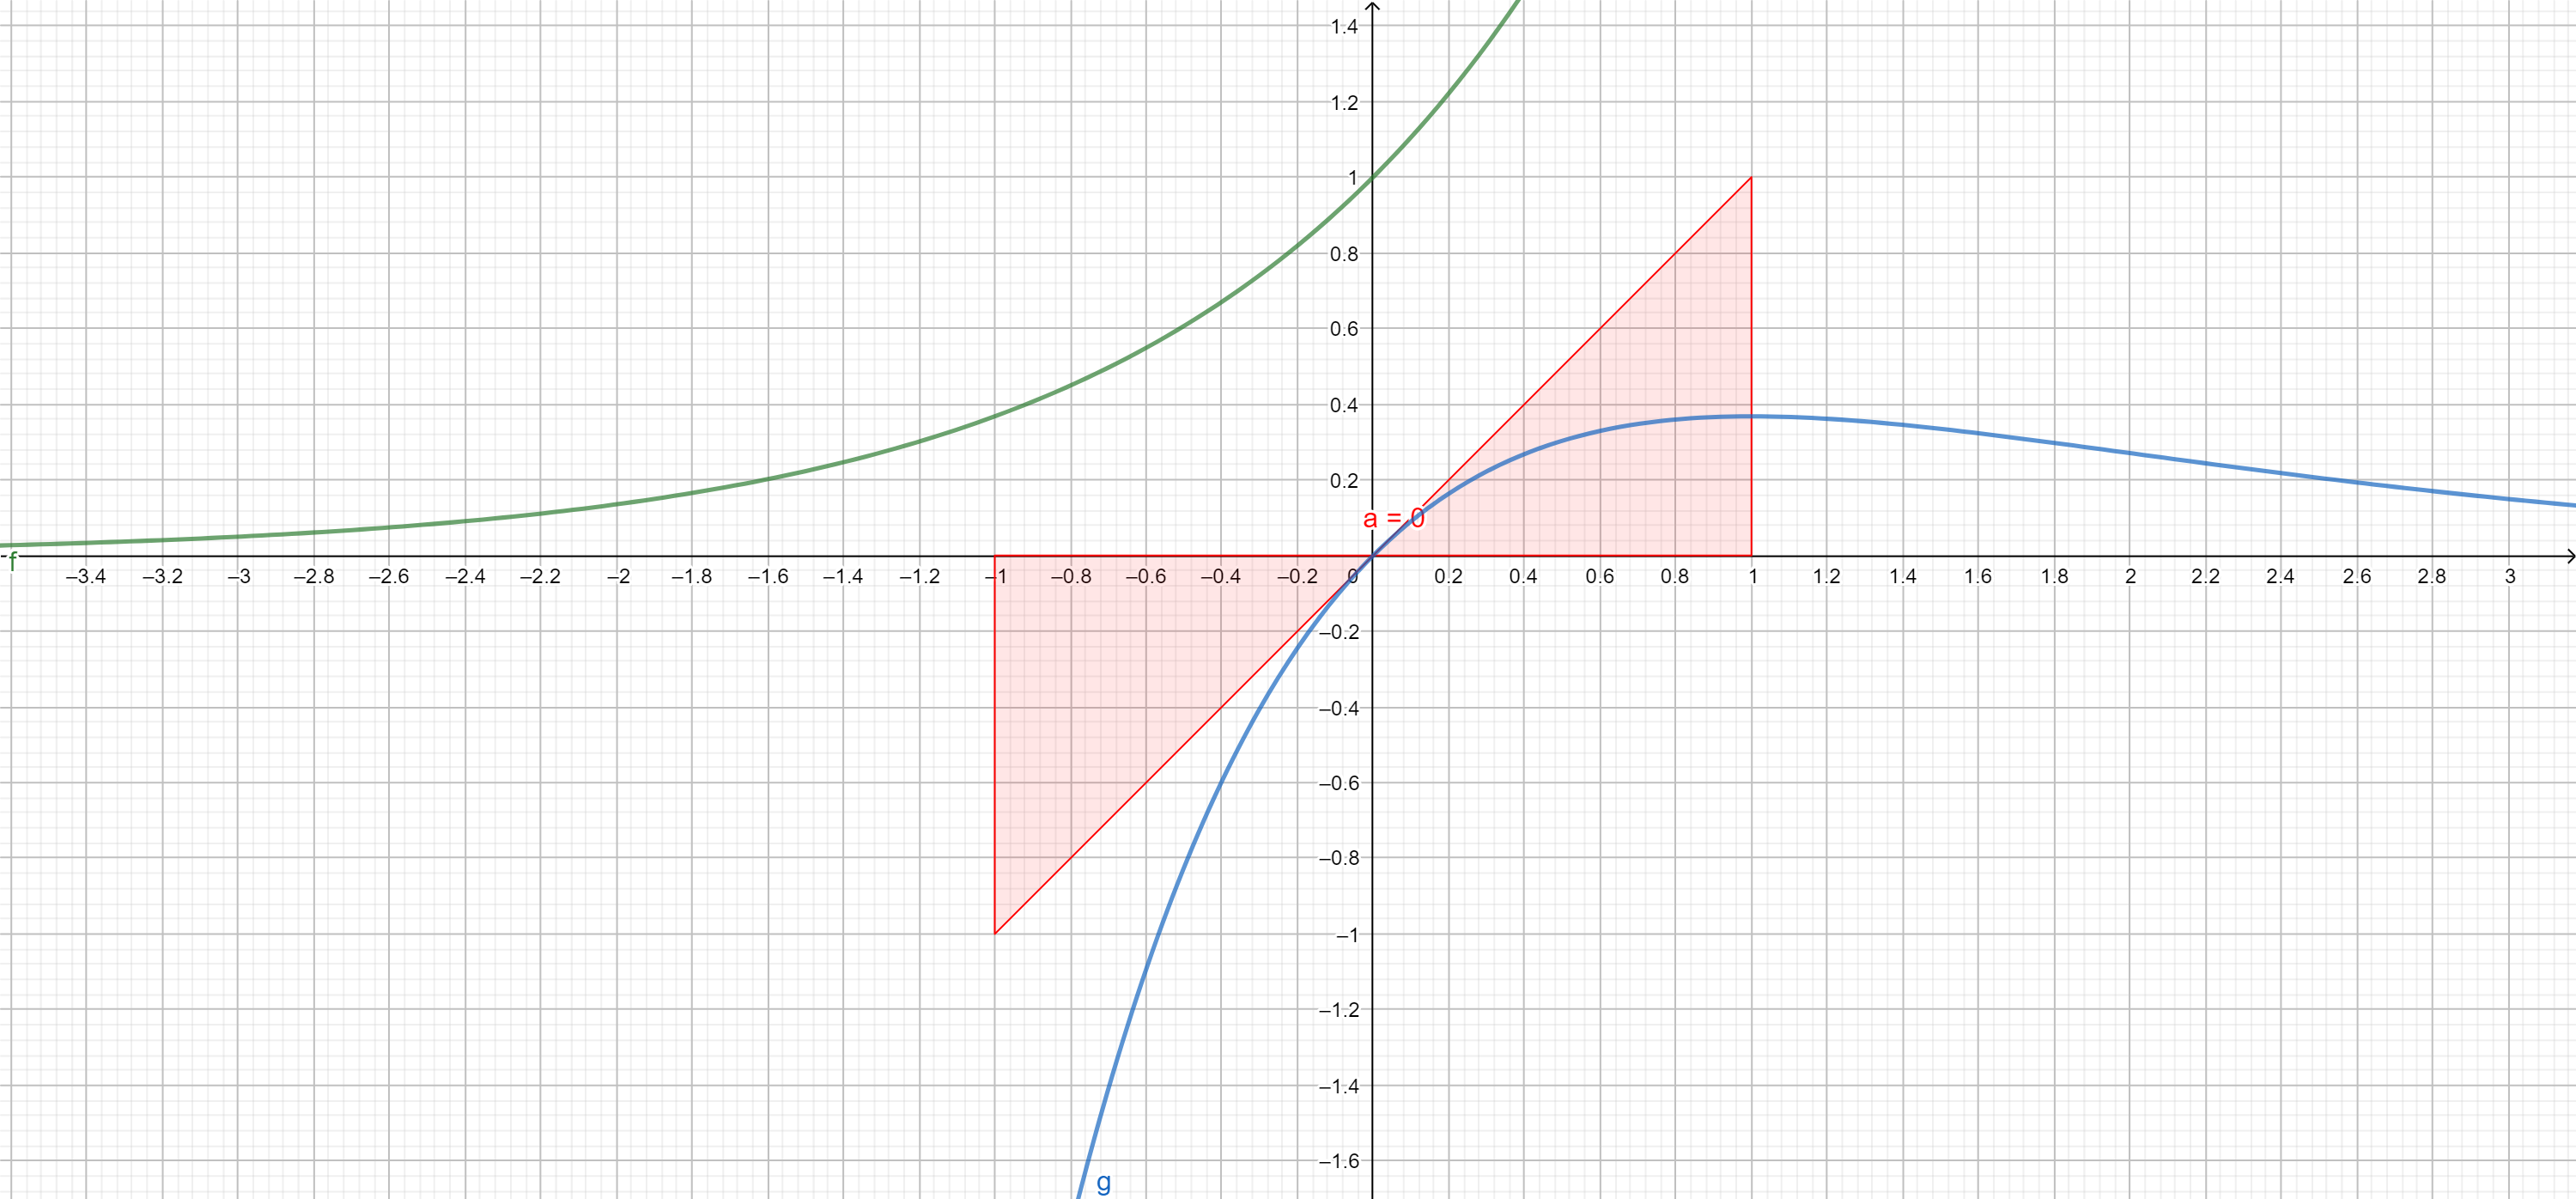
\includegraphics[width=\textwidth]{./img/inproduct functies.png}
    \caption{groen: f(x), blauw: g(x), rood: $\langle f,g\rangle$}
    \label{fig:orthofuncties}
\end{figure}

We zeggen dat $x,y$ orthogonaal op elkaar staan (in een Hilbertruimte) als $\langle x,y\rangle =0$.
De twee functies in het voorbeeld staan dus orthogonaal op elkaar. Functies die orthogonaal op elkaar staan hoeven elkaar dus niet loodrecht te snijden (zie figuur~\ref{fig:orthofuncties}).

In een Hilbertruimte wordt de lengte van $x$ gegeven door $||x||=\sqrt{\langle x,x\rangle}$.

\textbf{Voorbeeld:} De lengte van $f(x)=-3ix^4+5x^2+10i$ is $\sqrt{\langle f,f\rangle}$.
\begin{align*}
    \langle f,f\rangle
    &= \int_{-1}^1 f(x)\overline{f(x)}  dx\\
    &= \int_{-1}^1 (-3ix^4+5x^2+10i)(3ix^4+5x^2-10i) dx\\
    &= \int_{-1}^1 9x^8+35x^4+100 dx\\
    &= \left[x^9+7x^5+100x\right]_{-1}^1=216
\end{align*}
Dus $||f||=\sqrt{216}$.

\medskip
\begin{opdracht}
Laat het inproduct voor continue functies (die een reëel getal sturen naar een complex getal, bijvoorbeeld $e^{ix}$) gegeven zijn door $$\langle f,g\rangle=\int_{-1}^1 f(x)\overline{g(x)}dx.$$ met $\overline{g(x)}$ de complex geconjugeerde van $g(x)$, bijvoorbeeld $\overline{e^{ix}}=e^{-ix}$.
\begin{enumerate}
    \item Bereken $\langle f,g\rangle$ voor:
    \begin{align*}
        a.&\;& f(x)=x+4,g(x)=x^2+7\\
        b.&\;& f(x)=x^5+ix+7,g(x)=3x^3+2ix\\
        c.&\;& f(x)=\cos(x),g(x)=\tan(x)\\
        d.&\;& f(x)=e^{2\pi ix},g(x)=e^{4\pi ix}\\
    \end{align*}
%\end{enumerate}
%\end{opdracht}
%\begin{opdracht}
\item Gebruik hetzelfde inproduct als in de vorige opgave. Bereken $||f||$ voor:
    \begin{align*}
        a.\;& f(x)=5x+1
        & c.\;& f(x)=6e^x\\
        b.\;& f(x)=2ix^3+4x+1
        & d.\;& f(x)=e^{2\pi ix}
    \end{align*}
\end{enumerate}
\end{opdracht}
\begin{opdracht}
Laat het inproduct voor 2-dimensionale reële vectoren gegeven zijn door $$\langle x,y\rangle=x_1y_1+(x_2-x_1)(y_2-y_1).$$
\begin{enumerate}

\item Wanneer geldt $x_1y_1+(x_2-x_1)(y_2-y_1)=x_1y_1+x_2y_2$? (geef een voorbeeld).
\item Bereken $\langle x,y\rangle$ voor $x=\begin{pmatrix}2\\1\end{pmatrix}$ en $y=\begin{pmatrix}-1\\-3\end{pmatrix}$, en concludeer dat ze orthogonaal op elkaar staan.
\item Laat zien dat $x$ en $y$ niet loodrecht op elkaar staan (hoek van $90^\circ$).
\end{enumerate}
\end{opdracht}

\textbf{Projectie:} In een Hilbertruimte wordt de projectie van $x$ op $y$ (allebei niet nul) gegeven door $\frac{\langle x,y\rangle}{\langle y,y\rangle}y$.

\begin{center}

%\hspace{-24pt}
%\begin{minipage}{\textwidth}
    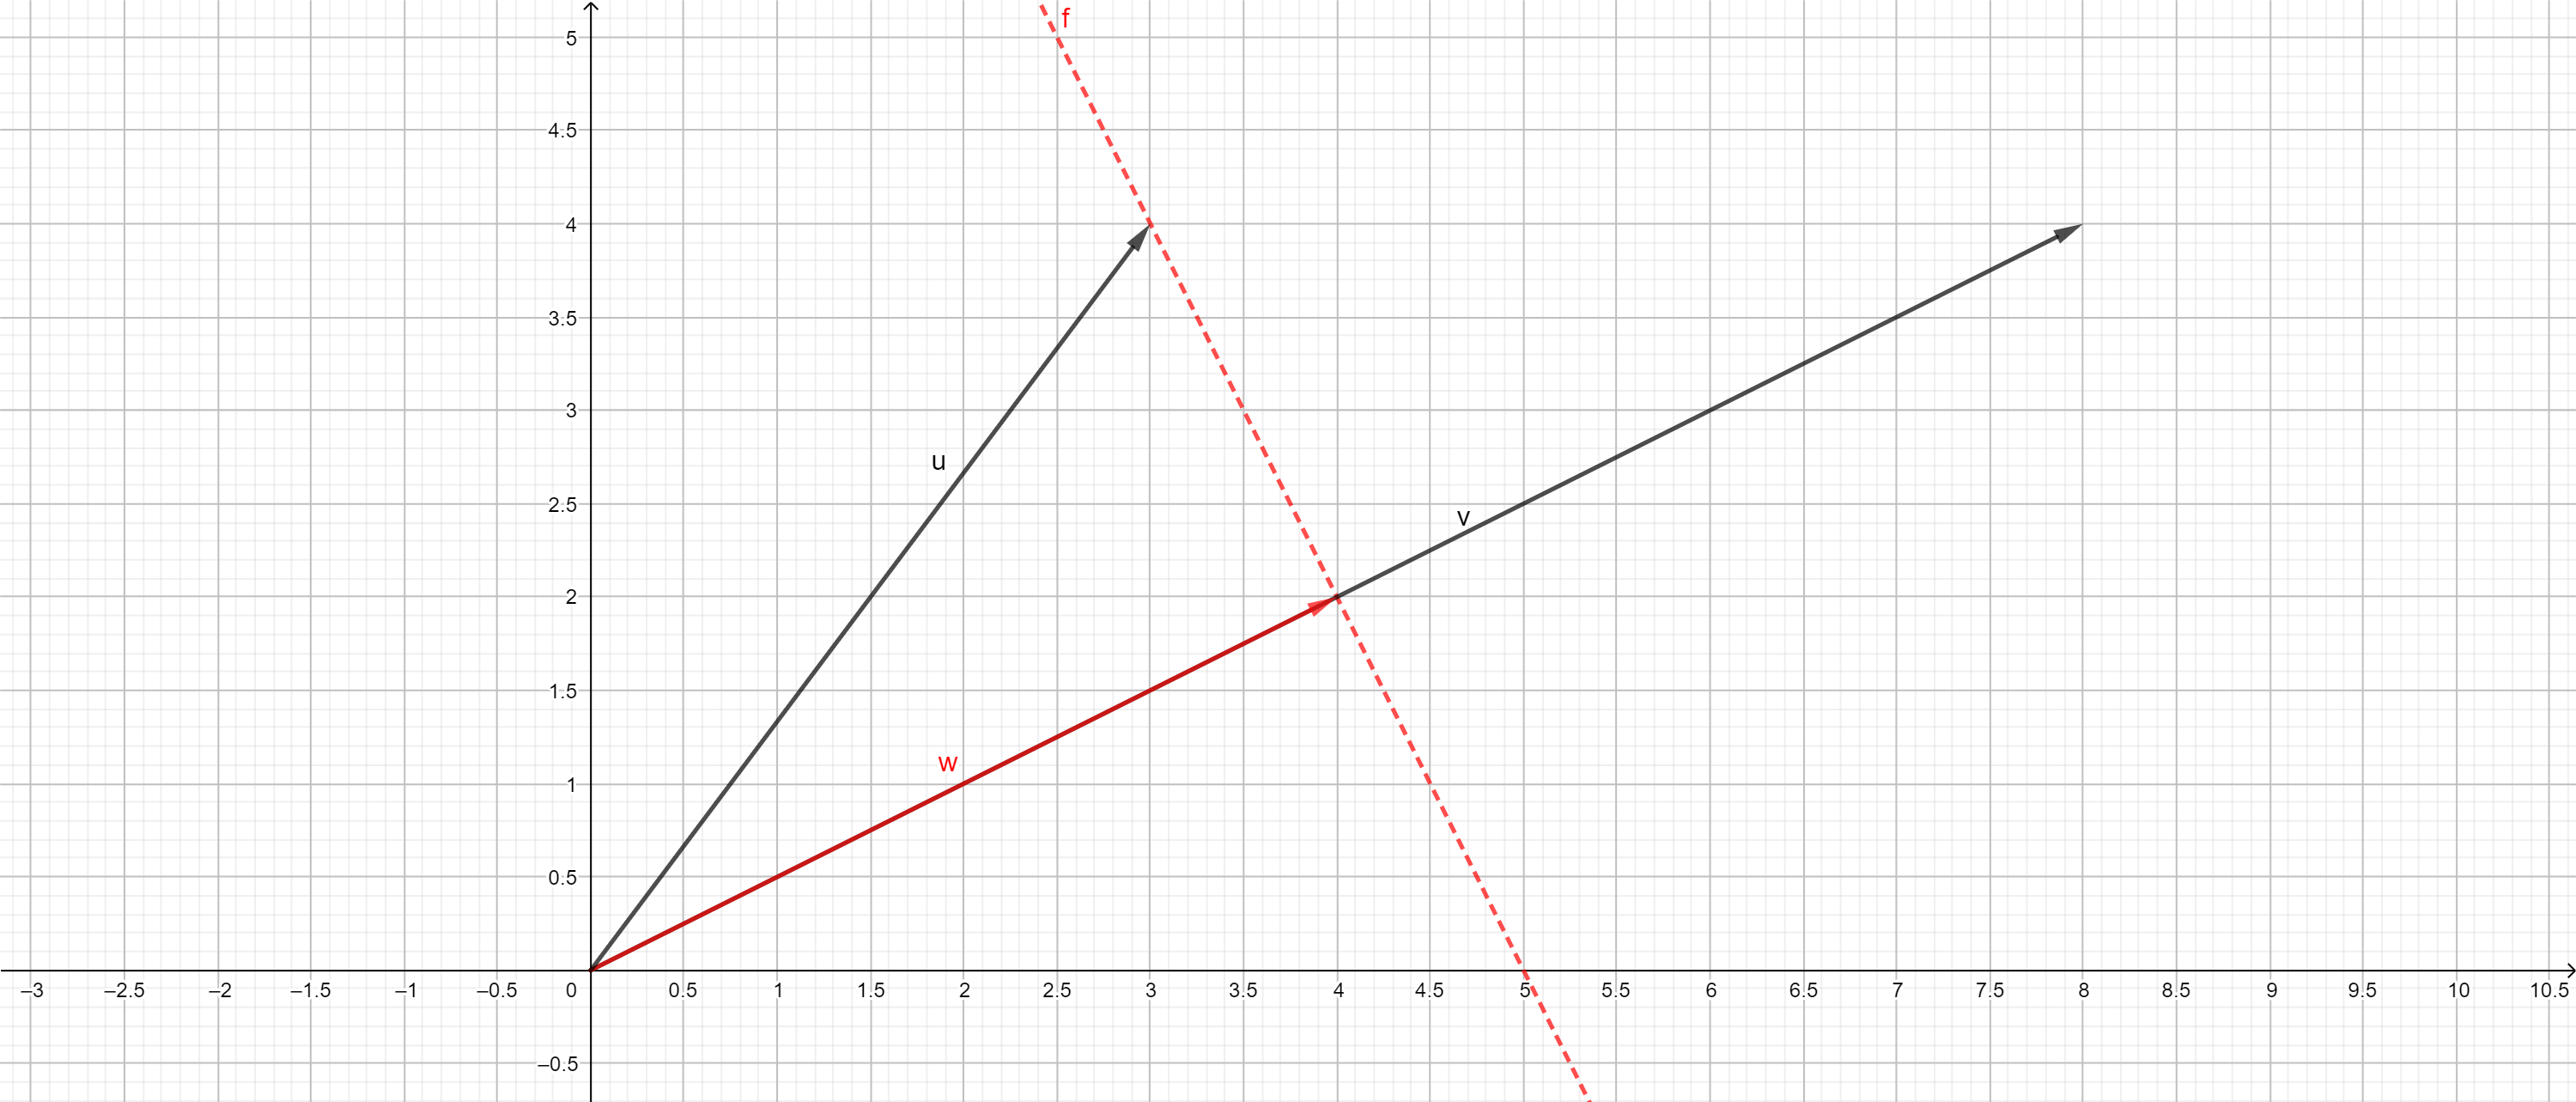
\includegraphics[width=\textwidth]{./img/projectie 1.png}
%\end{minipage}
\captionof{figure}{$w$ is de projectie van $u$ op $v$ (met behulp van een loodlijn). \label{fig:fig:loodlijn}}
\end{center}
\vspace{.5cm}

Dus de projectie van $x$ op $y$ is altijd in de vorm $\lambda\cdot y$ met $\lambda$ een getal.

\begin{opdrachtlang}\label{opd:hilbproj}
\begin{enumerate}
\item Bereken de projectie (met het standaard inproduct) van $x=\begin{pmatrix}5\\2\end{pmatrix}$ op $y=\begin{pmatrix}1\\0\end{pmatrix}$ (dit is de projectie van $x$ op de $y$-as).\\
\item\label{itm:inprodb} Laat het inproduct voor reële functies:
\[\langle f,g\rangle=\int_{1}^2 f(x)g(x)dx\]\\
Laat $f(x)=\frac{e^x}{x},g(x)=x^3+4x^2$ en $h(x)=x$. Bereken de projectie van $f(x)$ op $h(x)$, en bereken de projectie van $g(x)$ op $h(x)$\\
\item Schets de functies gevonden bij~\ref{itm:inprodb}.\\
\item Laat zien dat de projectie van $x$ op $x$ gelijk is aan $x$. 
\end{enumerate}
\end{opdrachtlang}

\begin{opdrachtlang}
Stel je hebt $x$ en $y$ (met $x$ niet een veelvoud van $y$), dan kun je $z$ vinden zodat $z$ en $y$ orthogonaal op elkaar staan. Een manier om dit te doen is de projectie van $x$ op $y$ uitrekenen en die van $x$ aftrekken. Dit geeft de formule $z=x-\frac{\langle x,y\rangle}{\langle y,y\rangle}y$.

%\hspace{-24pt}
\begin{minipage}{\textwidth}
    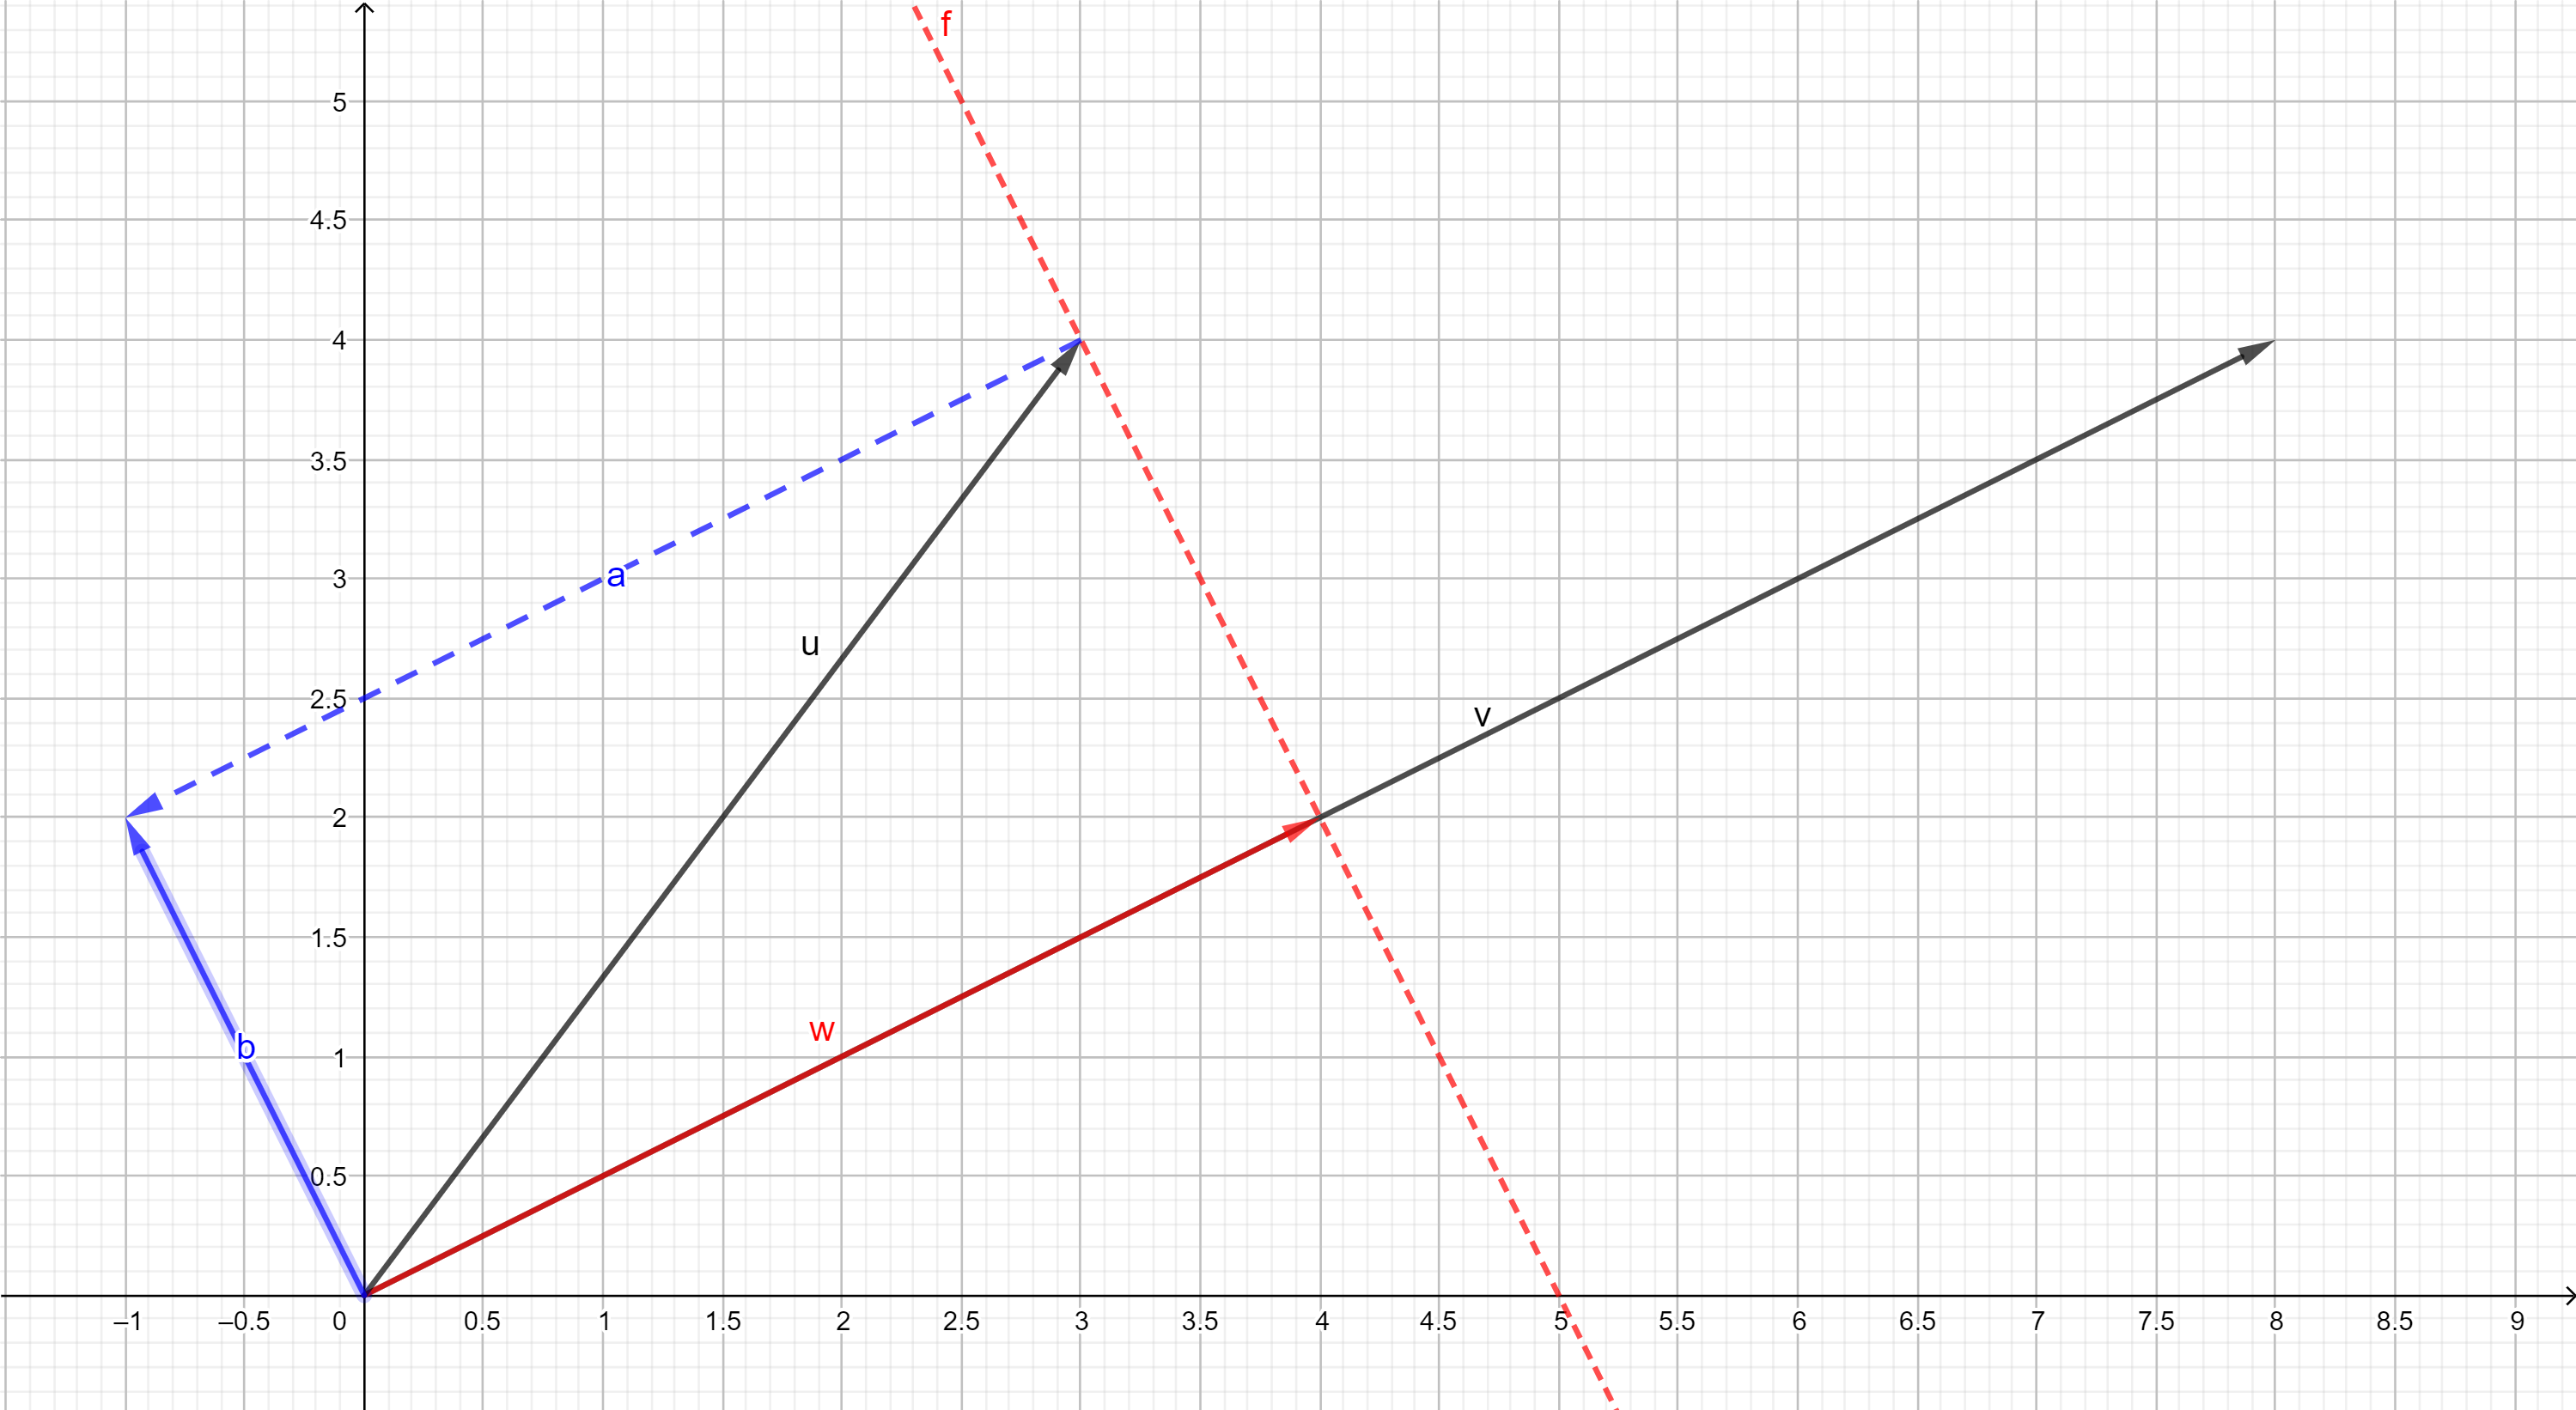
\includegraphics[width=.95\textwidth]{./img/projectie 2.png}
\end{minipage}
\captionof{figure}{b=u-w en inderdaad: $b$ staat loodrecht op v. \label{fig:fig:projectie}}
\vspace{.5cm}


%    \begin{figure}[h]
%    \centering
%    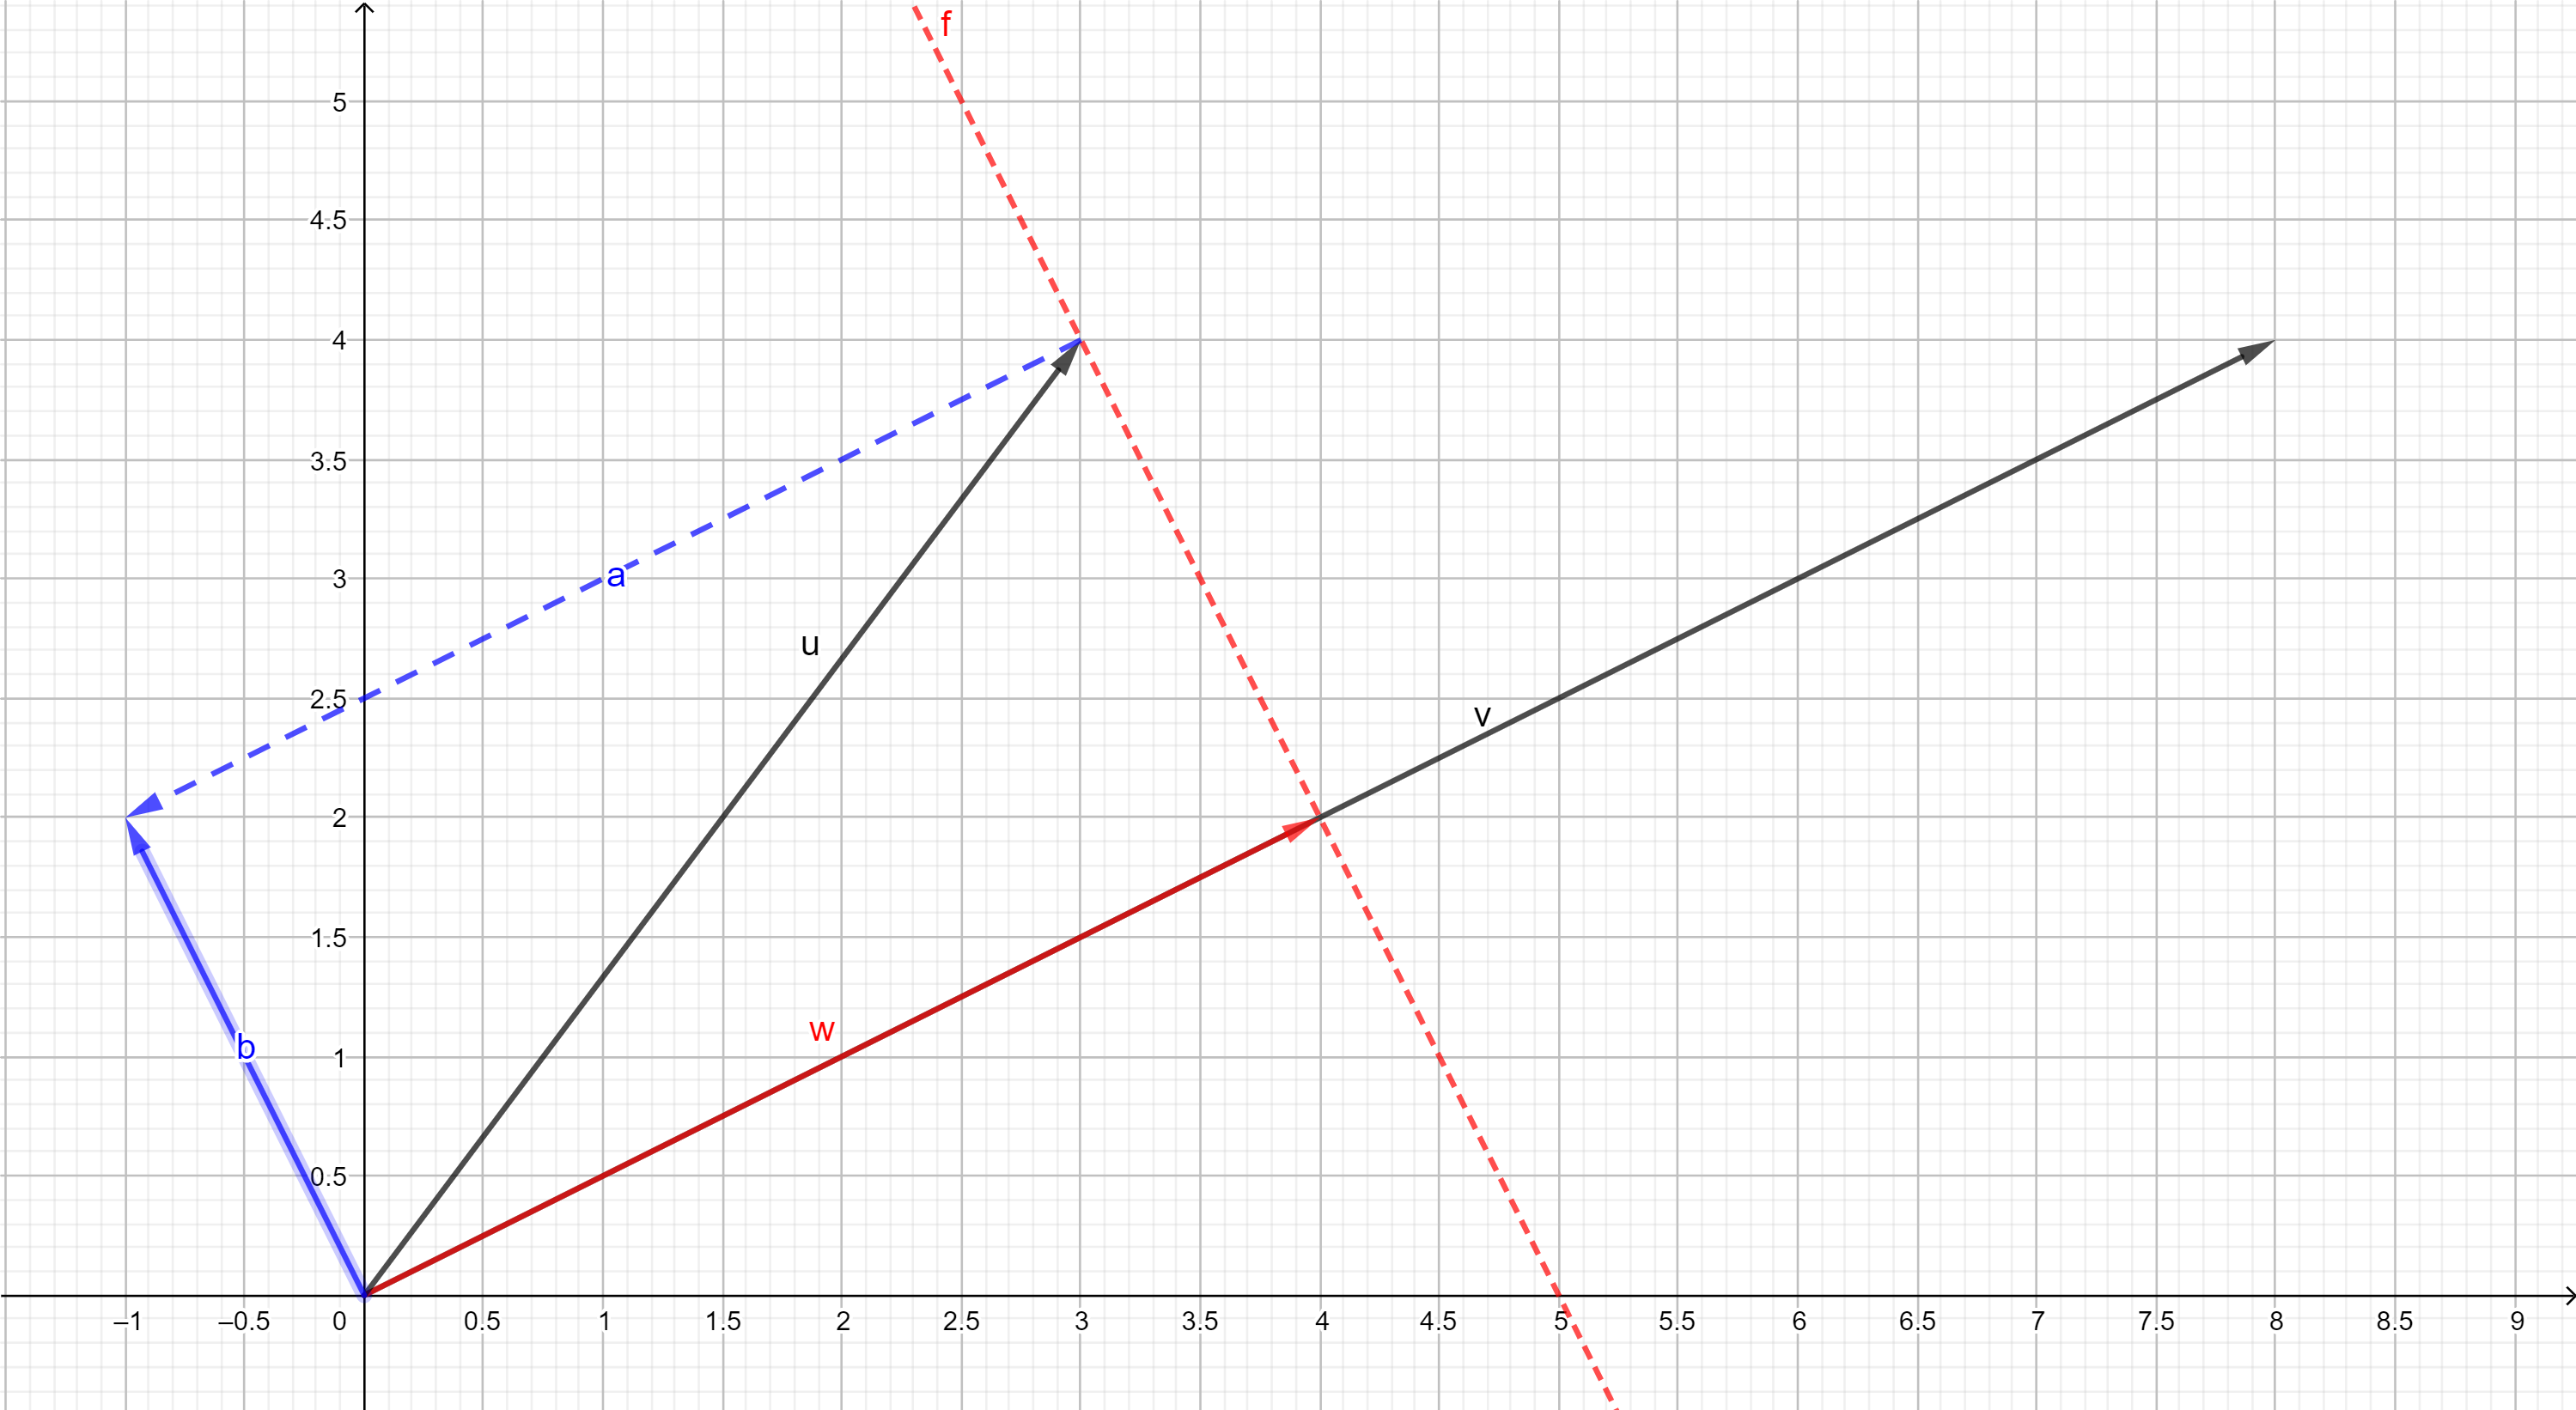
\includegraphics[scale=0.8]{./img/projectie 2.png}
%    \caption{b=u-w en inderdaad $b$ staat loodrecht op v}
%    \label{fig:my_label}
%\end{figure}


\begin{enumerate}
    \item Gebruik deze methode (met het standaard inproduct) om een orthogonaal element te vinden van $y=\begin{pmatrix}3\\1\end{pmatrix}$ met behulp van $x=\begin{pmatrix}7\\2\end{pmatrix}$. Ga na of de gevonden vector ook echt orthogonaal staat op $y$.
\item\label{itm:hilbfun} Laat het inproduct en de functies hetzelfde zijn als bij~\ref{itm:inprodb} van opdracht~\ref{opd:hilbproj}. Vind twee functies die orthogonaal staan op $h$.\\
\item Schets de functies gevonden bij ~\ref{itm:hilbfun}.
\end{enumerate}
\end{opdrachtlang}

\begin{opdracht}
\textbf{Pythagoras:} We gaan in deze opgave laten zien dat de stelling van Pythagoras geldt in elke Hilbertruimte.
\begin{enumerate}
\item Laat zien dat voor elk inproduct geldt $\langle x,\lambda_1y+\lambda_2z\rangle=\overline{\lambda_1}\langle x,y\rangle+\overline{\lambda_2}\langle x,z\rangle$ met $\lambda_1,\lambda_2$ complexe getallen. (hint: $\overline{a+b}=\overline{a}+\overline{b}$)
\item Schrijf $||x+y||^2$ uit en concludeer $||x+y||^2=\langle x,x\rangle+\langle x,y\rangle + \langle y,x\rangle+\langle y,y\rangle$
\item Laat zien dat als $\langle x,y\rangle=\langle y,x\rangle =0$ (dus $x$ en $y$ orthogonaal op elkaar staan), dat dan  $||x+y||^2=||x||^2+||y||^2$ (de stelling van Pythagoras).
\end{enumerate}
\end{opdracht}
Hilbert ruimten en Fourier analyse zijn twee van de vele wiskundige pijlers waarop de wiskunde van quantumcomputing is gebouwd.

\section{Fourieranalyse}

In de quantumtheorie spelen golven een belangrijke rol. Fourieranalyse probeert functies te koppelen aan golven. Voor de sinus is dat natuurlijk niet moeilijk want dat is al een golf, maar met Fourieranalyse kun je bijna alle functies zien als de som van golven, zelf functies zoals $\frac{1}{2}x$ kun je door maar een paar sinuso\"ides bij elkaar op te tellen erg goed benaderen. Ter voorbereiding hiervan zullen we eerst kijken naar een simpelere benaderingsmethode.

\subsection*{Taylorreeksen}
Zoals eerder gezegd kun je functies zien als vectoren (rijtjes getallen). In deze paragraaf laten we zien waarom dit zo is. We gaan proberen elke functie als een polynoom (bijvoorbeeld $x^4+3x^2+17$) te schrijven. Een voordeel hiervan is dat je door de eerste paar termen van het polynoom uit te rekenen al een zeer goede benadering krijgt van de functie (die ook nog makkelijk integreerbaar is). Voor een functie als $f(x)=x^9+5x^4+7$ is dat zeer makkelijk want dat is al een polynoom. We gaan nu proberen $f(x)=e^x$ te schrijven als het polynoom $$g(x)=a_0+a_1x+a_2x^2+a_3x^3+\ldots$$ Omdat $f(x)=g(x)$ en $f(0)=1$ geldt $g(0)=a_0=1$. Om $a_1$ uit te rekenen is het niet handig om een ander punt in te vullen want $$g(1)=a_0+a_1+a_2+\ldots$$ dit geeft geen makkelijke manier om $a_1$ uit te rekenen. Daarom gebruiken we de afgeleide $f'(x)=e^x$ dus $f'(0)=1$, maar $$g'(x)=a_1+2a_2x+3a_3x^2+4a_4x^3$$
dus $g'(0)=a_1=1$. Op dezelfde manier kun je door de afgeleide van $f'(x)$ (dus $f''(x)$) gebruiken om $a_2=\frac{1}{2}$ te vinden. Als je de eerste zes termen uitrekent krijg je: $$g(x)=1+x+\frac{1}{2}x^2+\frac{1}{6}x^3+\frac{1}{24}x^4+\frac{1}{120}x^5$$

\begin{figure}[h]
    \centering
    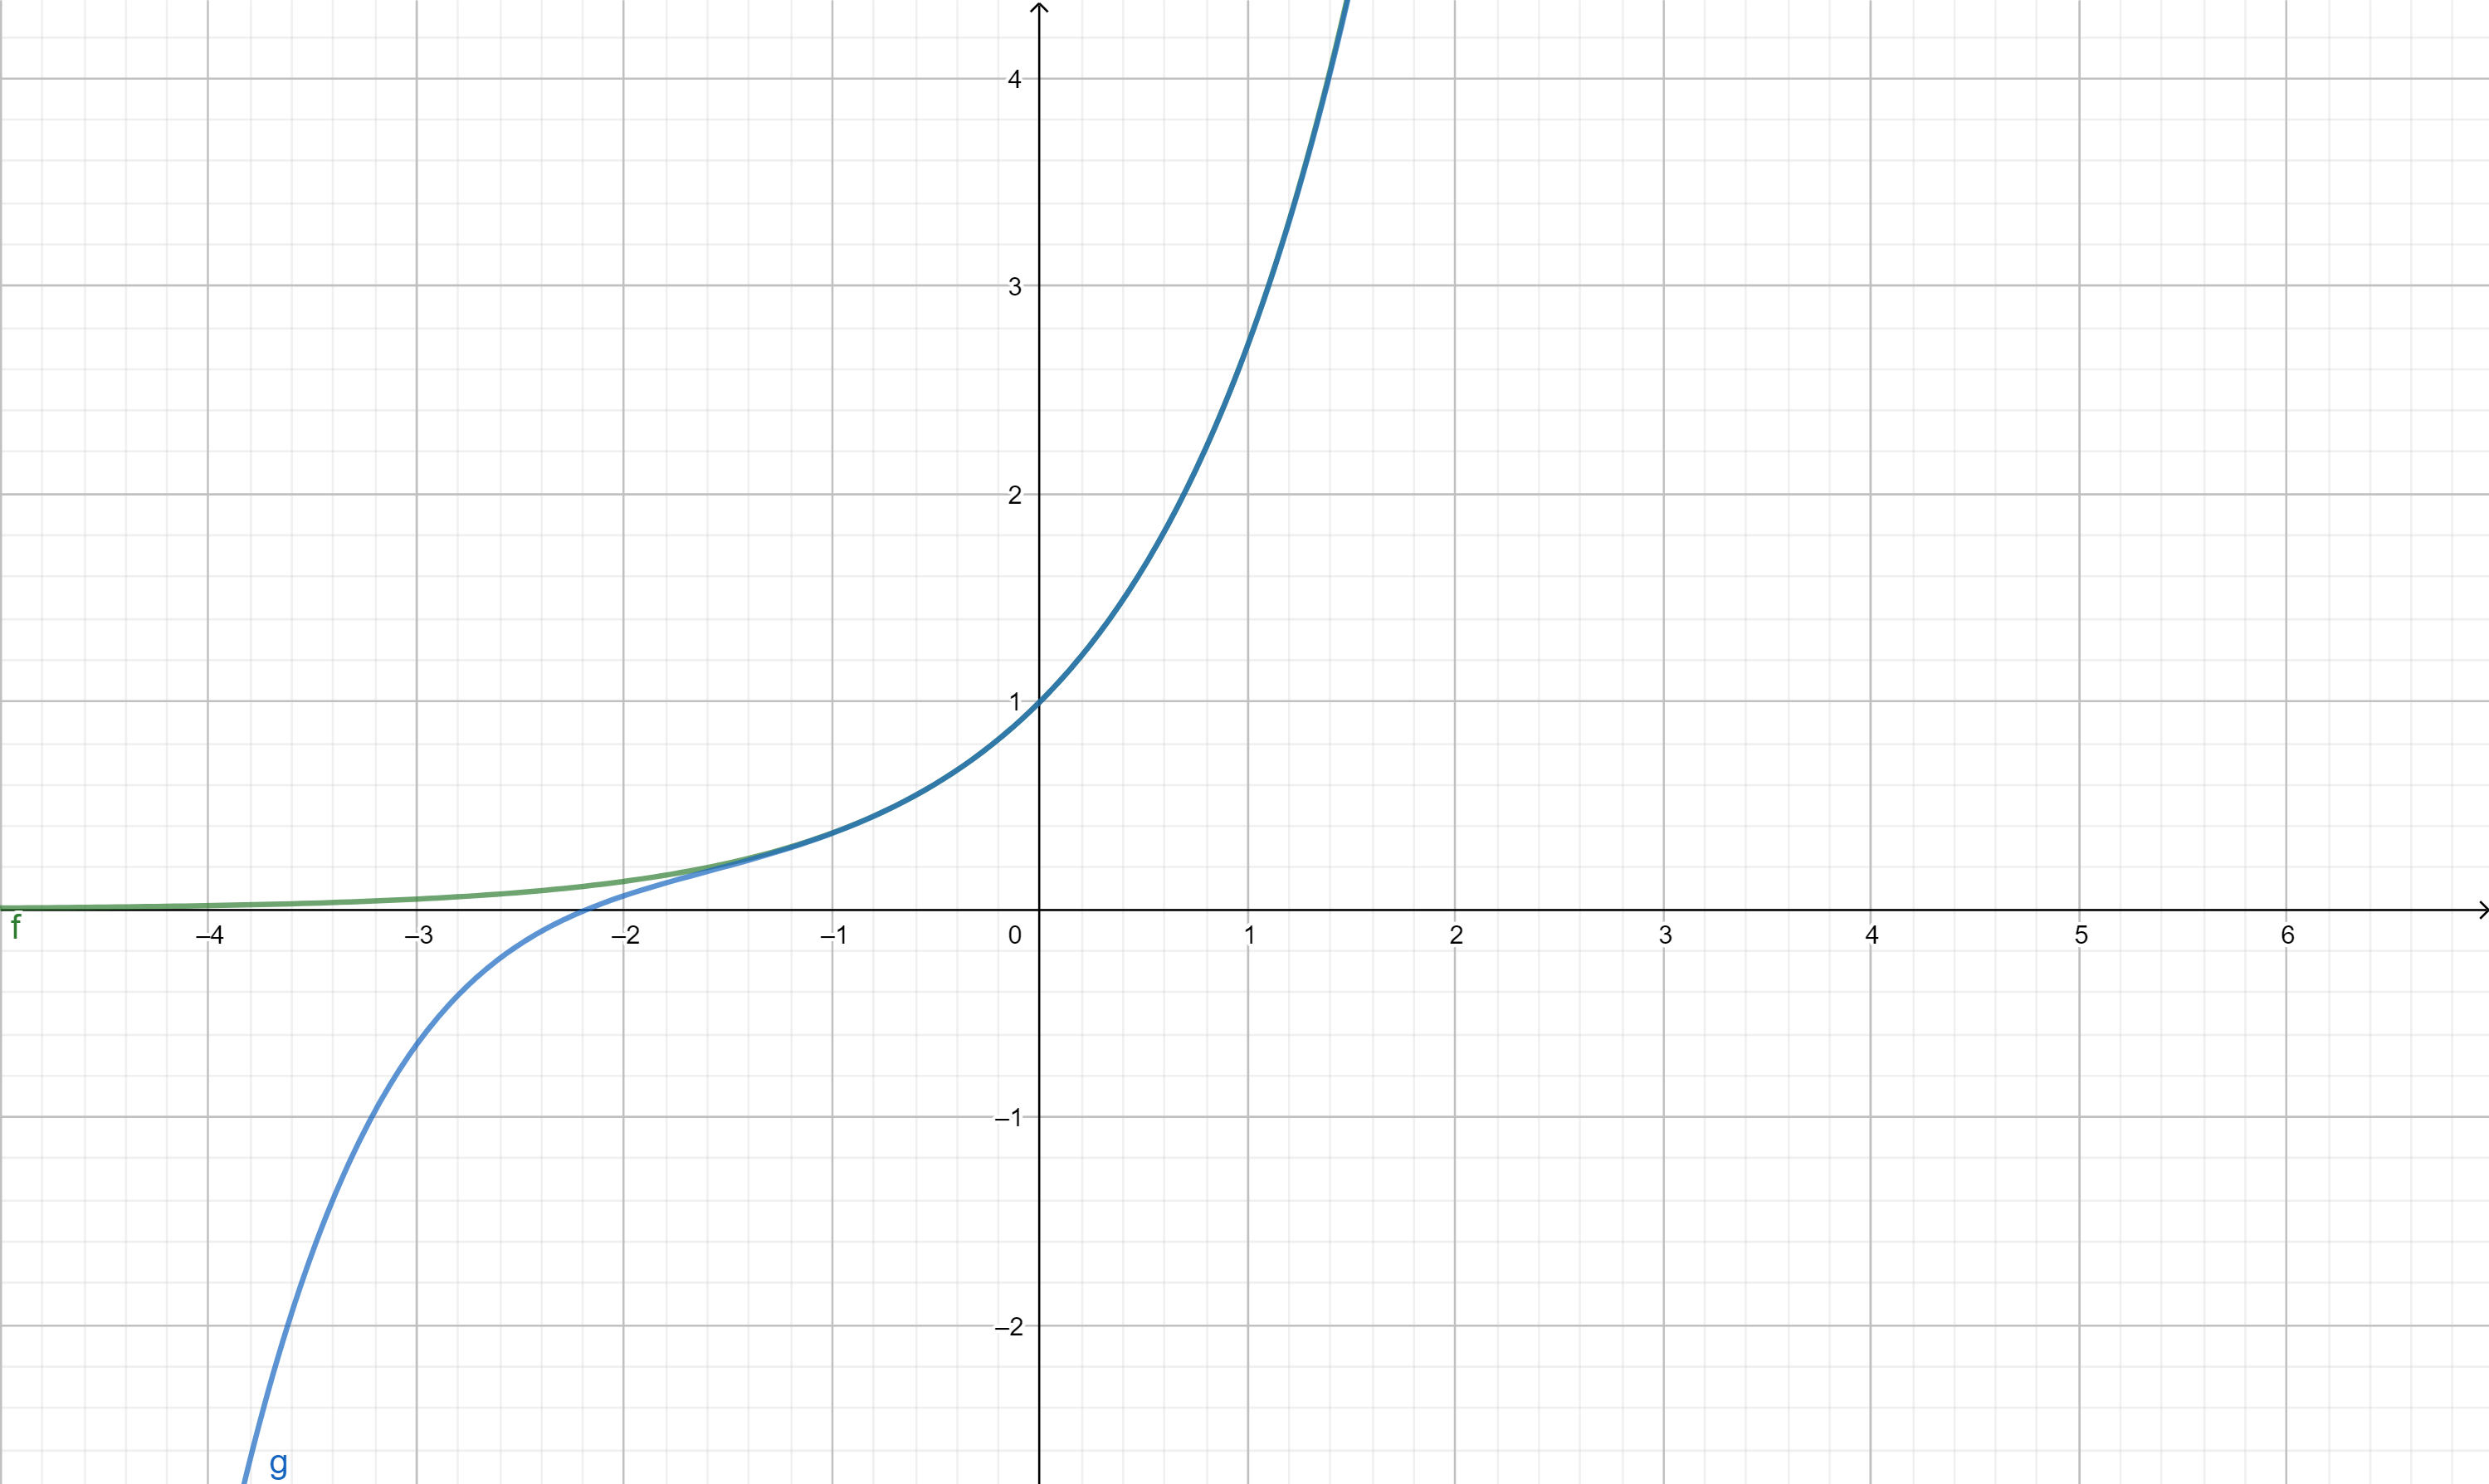
\includegraphics[width=\textwidth]{./img/taylor.png}
\end{figure}

Je ziet rond 0 dat $g$ een goede benadering is van $f$. Als je meer termen toevoegt zal de benadering steeds beter worden en als je oneindig veel termen hebt zijn $g$ en $f$ gelijk.\\
De algemene formule van een Taylorreeks (rond 0) voor een functie $f$ is $$g(x)=f(0)+f^{(1)}(0)x+\frac{f^{(2)}(0)}{2!}x^2+\frac{f^{(3)}(0)}{3!}x^3+\frac{f^{(4)}(0)}{4!}x^4+\ldots$$
Hierbij is $f^{(n)}(0)$ de $n-$de afgeleide in 0 dus $f^{(2)}(0)=f''(0)$ en $n!=1\cdot2\cdot3\cdot\ldots\cdot n$ dus $4!=1\cdot2\cdot3\cdot4=24$ ($0!=1$).\\
We bekijken weer $f(x)=e^x$ omdat ook $f'(x)=e^x$. Er geldt $f^{(n)}(0)=e^0=1$ dus $$g(0)=1+x+\frac{1}{2!}x^2+\frac{1}{3!}x^3+\frac{1}{4!}x^4+\ldots$$
Je kunt $e^x$ dus zien als de rij getallen $(1,\frac{1}{2!},\frac{1}{3!},\frac{1}{4!},\ldots)$.

\begin{opdracht}
\begin{enumerate}
    \item Bereken de eerste 4 termen van de Taylorreeks van de volgende functies en plot $f$ en $g$

     \begin{align*}
        a.\;& f(x)=x^5+2x^4+3x^2+12x+3
        & c.\;& f(x)=2e^{2x}\\
        b.\;& f(x)=\sin(x)
        & d.\;& f(x)=e^{x^2}
    \end{align*}
\end{enumerate}
Als je een Taylorreeks probeert te maken van $f(x)=\frac{1}{x}$ heb je een probleem want $f(0)$ is niet gedefinieerd.
\begin{enumerate}[resume]
    \item Vervang $x$ door $x=y+1$ en bereken $f^{(1)}(y),f^{(2)}(y)$ en $f^{(3)}(y)$.
    \item Bepaal de eerste 4~termen van de Taylorreeks van $f(y)$.\\
    \item Substitueer $y=x-1$ in de Taylorreeks en plot $f$ en $g$\\
    \item Gebruik dezelfde truc om een benadering te maken (4~termen) van $f(x)=\ln(x)$.
\end{enumerate}
\end{opdracht}

\subsection*{Fourierreeksen}
In deze paragraaf gaan we een andere benadering vinden van (periodieke) functies aan de hand van sinusoïde. Hiervoor gebruiken we het volgende inproduct: \[\langle f,g\rangle=\frac{1}{2\pi}\int_{0}^{2\pi} f(x)g(x)dx.\]
Als benadering voor de functie $f$ gebruiken we nu de volgende functie 
\begin{align*}
    g(x)=&a\\
    &+b_1\sin(x)+b_2\sin(2x)+b_3\sin(3x)+\ldots\\
    &+c_1\cos(x)+c_2\cos(2x)+c_3\cos(3x)+\ldots
\end{align*}
Als we proberen $a$ uit te rekenen (op dezelfde manier zoals bij Taylorreeksen) komen we in de problemen, want als $\sin(x)=0$ dan $\cos(x)\neq 0$. 
Daarom gebruiken we dat als $f=g$ dat dan de projectie $P$ op $h(x)=1$ voor $f$ en $g$ hetzelfde zijn.
\begin{align*}
    P(x)&=\frac{\langle g,h\rangle}{\langle h,h\rangle}h\\
    &=\langle a,h\rangle+\langle b_1\sin(x),h\rangle+\langle c_1\cos(x),h\rangle+\ldots
\end{align*}
maar omdat $h(x)=\cos(0x)$ is $h$ een sinusoïde dus staat $h$ orthogonaal op alle andere sinusoïde. Dus\\
\begin{align*}
    P(x)&=\langle a,h\rangle\\
    &=\frac{1}{2\pi}\int_0^{2\pi}adx=a
\end{align*}
Ook geldt \begin{align*}
    P(x)&=\frac{\langle f,h\rangle}{\langle h,h\rangle}h\\
    &=\frac{1}{2\pi}\int_0^{2\pi}f(x)dx
\end{align*}
Dus $$a=\frac{1}{2\pi}\int_0^{2\pi}f(x)dx=\langle f,1\rangle$$.\\
Op dezelfde manier geldt\begin{align*}
     b_n&=\frac{1}{2\pi}\int_0^{2\pi}f(x)\sin(nx)dx=\langle f,\sin(nx)\rangle\\ 
     c_n&=\frac{1}{2\pi}\int_0^{2\pi}f(x)\cos(nx)dx=\langle f,\cos(nx)\rangle.\\
     \end{align*}
Als voorbeeld bekijken we $f(x)=\frac{1}{2}x$ waarvoor dan geldt 
\begin{align*}
    a&=\frac{1}{2\pi}\int_0^{2\pi}\frac{1}{2}xdx=\frac{1}{2\pi}\left[\frac{1}{4}x^2\right]_0^{2\pi}=\frac{\pi}{2}\\
    b_1&=\frac{1}{\pi}\int_0^{2\pi}\frac{1}{2}x\sin(x)dx=\frac{1}{\pi}\left[\frac{1}{2}\sin(x)-\frac{1}{2}x\cos(x)\right]_0^{2\pi}=-1\\
    c_1&=\frac{1}{\pi}\int_0^{2\pi}\frac{1}{2}x\cos(x)dx=\frac{1}{\pi}\left[\frac{1}{2}x\sin(x)+\frac{1}{2}\cos(x)\right]_0^{2\pi}=0
\end{align*}
Dus we krijgen als benadering $g(x)=\frac{\pi}{2}-\sin(x)$.
\begin{figure}[h]
    \centering
    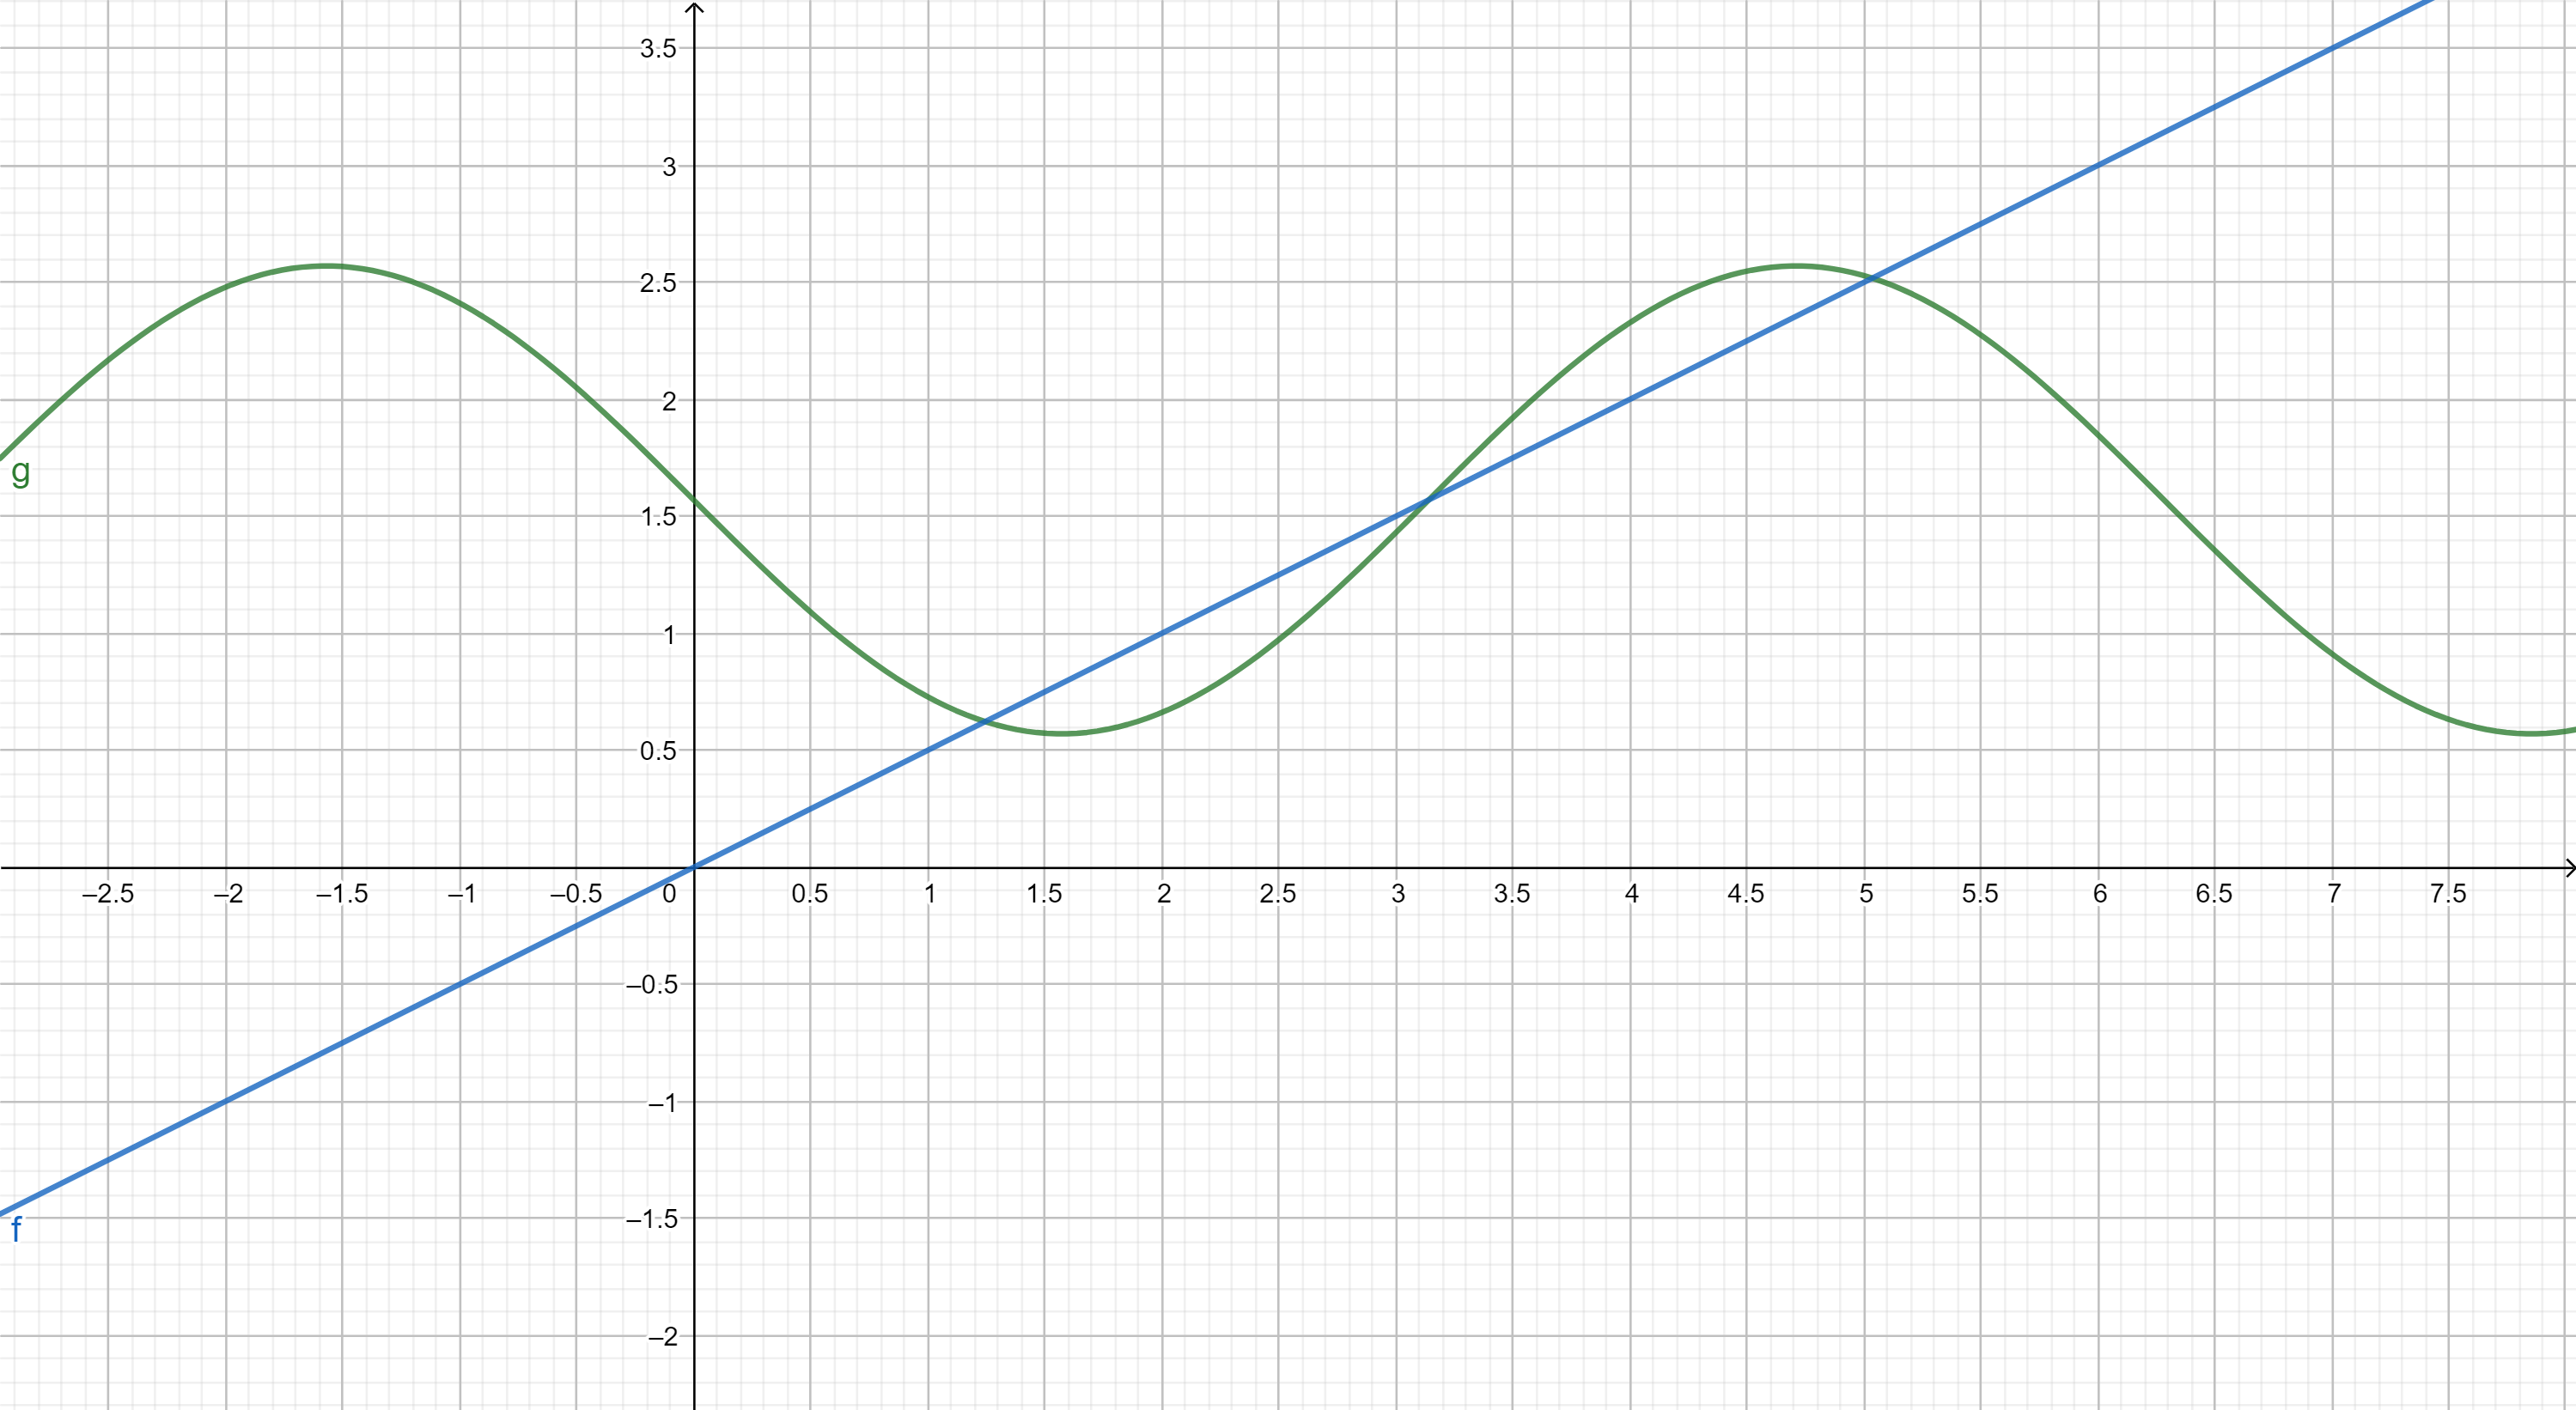
\includegraphics[width=\textwidth]{./img/fourier_1.png}
\end{figure}

Zoals je ziet is het nog niet zo 'n goede benadering. Als je $b_2$ tot en met $b_5$ \ en $c_2$ tot en met $c_5$ uitrekent krijg je:
$$g(x)=\frac{\pi}{2}-\sin(x)-\frac{1}{2}\sin(2x)-\frac{1}{3}\sin(3x)-\frac{1}{4}\sin(4x)-\frac{1}{5}\sin(5x)$$
\begin{figure}[h]
    \centering
    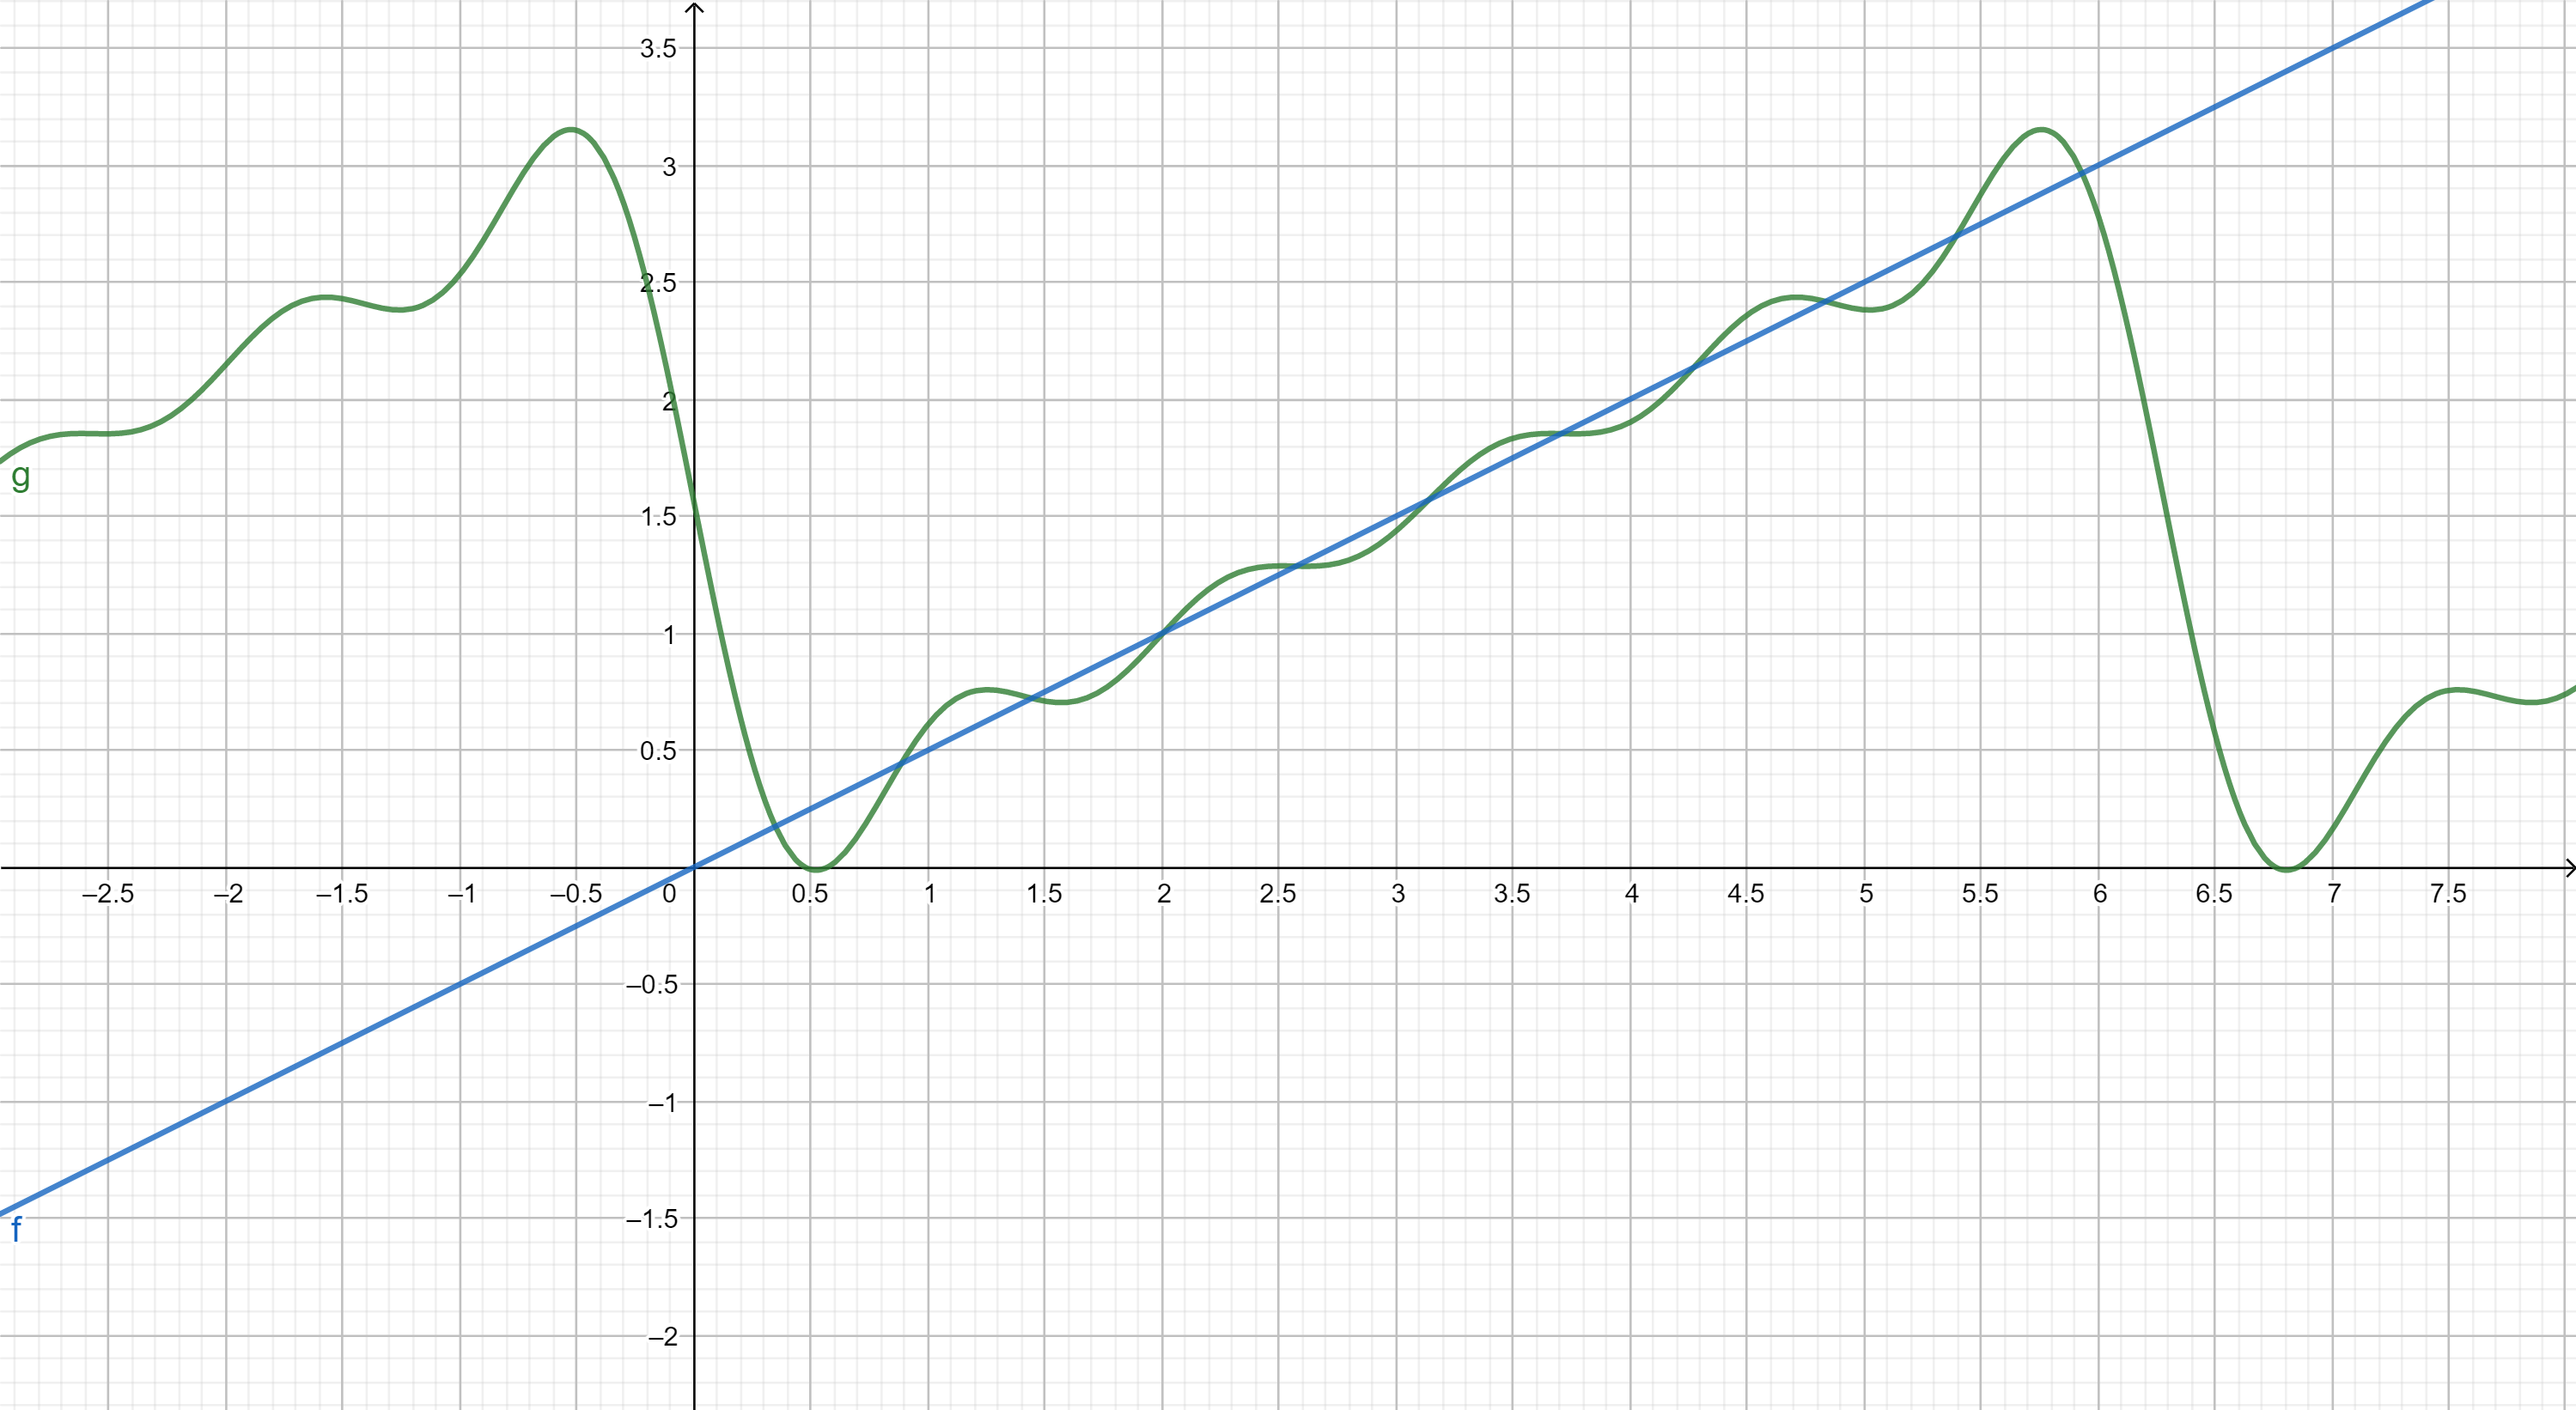
\includegraphics[width=\textwidth]{./img/fourier_2.png}
\end{figure}

Dit is al een veel betere benadering, maar alleen in het interval $(0,2\pi)$ daarna herhaalt de grafiek zich. Dit blijft het geval hoeveel termen je ook uitrekent daarom is deze manier juist geschikt voor periodieke functies.

\begin{opdrachtlang}
\begin{enumerate}
    \item Laat zien dat $\int \sin(2x)\cos(x) dx=-\frac{2}{3}\cos^3(x)$.\\
    \item Laat zien dat $\sin(2x)$ en $\cos(x)$ orthogonaal op elkaar staan (met het hierboven genoemde inproduct).
    \item Bereken $a, b_1,b_2,c_1$ en $c_2$ van de Fourierreeks van de volgende functies (met behulp van je GR) en plot $f$ en $g$. \begin{align*}
        a.\;& f(x)=x^2-x-1
        & c.\;& f(x)=e^{x}\\
        b.\;& f(x)=\tan(\frac{x-\pi}{2})
        & d.\;& f(x)=\frac{1}{x+1}
    \end{align*}
\end{enumerate}

We kunnen ook een ander inproduct nemen voor een fourierreeks. Beschouw \[\langle f,g\rangle=\frac{1}{4\pi}\int_{-2\pi}^{2\pi} f(x)g(x)dx\]

Net als hiervoor zoeken we een benadering voor een functie $f$ en die benadering is nog steeds
    \begin{align*}
        g(x)=&a\\
        &+b_1\sin(x)+b_2\sin(2x)+b_3\sin(3x)+\ldots\\
        &+c_1\cos(x)+c_2\cos(2x)+c_3\cos(3x)+\ldots
    \end{align*}
\begin{enumerate}[resume]
\item Laat zien met behulp van projectie dat $a=\langle f,1\rangle$.
\end{enumerate}

Er geldt $b_n=\langle f,\sin(nx)\rangle$ en $c_n=\langle f,\cos(nx)\rangle$. 
\begin{enumerate}[resume]
\item Bereken $a, b_1,b_2,c_1$ en $c_2$ van de Fourierreeks van de volgende functies (met behulp van je GR) en vergelijk met de antwoorden gevonden bij opgave $2$.
   \begin{align*}
a.\;& f(x)=x^2-x-1.\\
b.\;& f(x)=e^x.\\
    \end{align*}
    
\end{enumerate}
\end{opdrachtlang}
Fouriertransformaties hebben tal van toepassingen in het dagelijks computerleven. Bijvoorbeeld in geluids- en beeldverwerking. Quantum Fouriertransformaties zijn ook een essentiele stap in het algoritme van Shor, waarmee grote getallen kunnen worden ontbonden in priemfactoren. Je begrijpt dat de bancaire sector en internet giganten in dit vakgebied belangrijke spelers zijn.

\iffalse%-even op een zijsppoor----

\nogdoen{niet kwijtraken! hier is een groot stuk tekst uitgecommentarieerd met materiaal voor talloze opdrachten}

\section{Protocol: Deutsch-Josza}\label{sec:poDeutsch}
Een van de eerste algoritmen die aantoonden dat een quantumcomputer iets kan dat een  klassieke computer niet kan.
\nogdoen{zie spelletjes}


\section{Kenniscentra}
Universiteiten en hogescholen bij jou in de buurt bieden ondersteuningsprogramma's aan. Het is d\'e manier om kennis te maken met je vervolgopleiding... \nogdoen{dit is van wat langere adem activiteiten in Amsterdam, Delft Eindhoven Twente Leiden en elders .informatie tzt op de website van het project..}


\section{Hoe bouw je een quantumcomputer}\label{sec:pobouwqc}
Er komt meer bij kijken om quantumcomputer te bouwen. In deze opdracht krijg je inzicht in de technologische uitdagingen waar jullie voor staan. \nogdoen{wordt aan gewerkt.}



\section{Alleen op een eiland oud}
\nogdoen{oude versie kan weg}Alice woont op een verder onbewoond eiland. Ze heeft met niemand contact, behalve met Bob, die ze berichten kan sturen als er dingen misgaan op het eiland. Alice kan Bob alleen klassieke bits sturen. Ze hebben de volgende codering afgesproken: 

\vspace*{12pt}
{\footnotesize
\begin{tabular}{r|l}
11 & Er is geen voedsel op het eiland\\\hline 
10 & Er is droogte. Geen water op het eiland\\\hline  
01 & Nieuw materiaal voor mijn huisje nodig \\\hline 
00 & SOS!
\end{tabular}
}
\vspace*{12pt}

Alleen als Bob een volledige code ontvangt, kan hij Alice helpen. Alice kan de bits slechts een voor een versturen. Alice begint altijd met beide bits in 0 (00). 
\begin{antwoord}
a) NOT(0)=>1,I(0)=>0\\
b) 2
\end{antwoord}
\begin{enumerate}
\item Er is een droge periode geweest en Alice heeft dringend water nodig. Welke klassieke poort(en) moet ze toepassen op welke bits om de boodschap aan Bob door te geven? 
\item Wat is het minimale aantal bits dat Alice aan Bob moet versturen om een boodschap door te geven?
\end{enumerate}
Alice en Bob gaan met hun tijd mee en hebben besloten over te stappen op quantumcommunicatie. Ze delen twee volledig verstrengelde qubits in een van de Bell-toestanden. Bedenk je dat er vier Bell toestanden zijn:

G: $\alpha\ket{00}+\beta\ket{11}$\\
H: $\alpha\ket{00}-\beta\ket{11}$\\
J: $\alpha\ket{10}+\beta\ket{01}$\\
K: $\alpha\ket{10}-\beta\ket{01}$\\
Alice en Bob delen een Bell toestand (toestand G van hierboven). 

\begin{antwoord}
c) toestanden zijn niet te isoleren door ontbinging $\alpha\ket{0}+\beta\ket{1}$\\
d) GH: ook een 0; JK juist een 1\\

\end{antwoord}
\begin{enumerate}[resume]
\item \label{enum:classic}Hoe kun je zien dat deze toestanden (bijvoorbeeld G) verstrengeld zijn? 
\item Als Alice een meting doet en ze meet 0, wat zal Bob dan als uitkomst van een meting krijgen? 
\item Zwarte piste? Wat is de kans dat Alice 0 meet? 
\end{enumerate}
\begin{enumerate}[resume]
\item Stel, Alice doet een X-rotatie op haar qubit, wat gebeurt er dan met haar qubit? En met Bob's qubit? Schrijf de nieuwe verstrengelde toestand op. 
\item Welke quantumpoort moet Alice op haar qubit toepassen om de toestand H te krijgen? 
\item Kun je bedenken met welke poort(en) Alice de toestand $\frac{\ket{01}-\ket{10}}{\sqrt{2}}$,(K) krijgt? 
\item Alice en Bob willen, in plaats van de klassieke bits, kijken of ze deze verstrengelde toestand kunnen gebruiken om hun communicatie mee te doen. Ze hebben dus elk \'e\'en van de twee verstrengelde qubits. Als Alice iets nodig heeft, kan ze haar qubit naar Bob sturen en meet Bob de verstrengelde toestand. Kun je een strategie bedenken waarmee Alice en Bob nu kunnen communiceren?

\item Hoeveel (qu)bits moet Alice nu naar Bob sturen om een boodschap door te geven? Wat is hier bijzonder aan (vergelijk je antwoord met vraag~\ref{enum:classic}).
\end{enumerate}

\section{Teleportatie}
\marginpar{\nogdoen{deze versie in doc handleiding, wordt ingekort voor leeringenversie }}
In science fictie komt teleportatie veelvuldig voor. Veelal wordt er een machine gebruikt die een persoon ergens laat verdwijnen en vervolgens op een totaal andere locatie laat verschijnen. Bij quantumteleportatie worden geen voorwerpen geteleporteerd, maar de informatie van een qubit; door slim gebruik te maken van verstrengeling, wordt bij teleportatie een qubit op plek A gemeten, verdwijnt de informatie en wordt de qubit op plaats B gereconstrueerd, zonder de qubit daadwerkelijk naar plaats B te sturen.
\begin{antwoord}
a)c\\
b)b\\
c)ja, $\alpha^2+\beta^2=1$\\
d)??
\end{antwoord}
\begin{enumerate}
\item Als je een qubit meet die in de toestand $\alpha\ket{0}+\beta\ket{1}$ is, meet. Wat is dan de uitkomst van de meting?
\begin{itemize}
\item 0
\item 1
\item 0 met kans $|\alpha|^2$ en 1 met kans $|\beta|^2$ 
\item iets tussen 0 en 1 in
\end{itemize}
\item Wat gebeurt er als je een verstrengelde qubit uit de toestand  $\frac{\ket{00}+\ket{11}}{\sqrt{2}}$ meet?
\begin{itemize}
\item De uitkomst van de qubits is altijd tegengesteld: als jij $\ket{0}$ meet, zal de andere qubit altijd $\ket{1}$ zijn.
\item De uitkomst van de qubits is altijd gelijk als jij $\ket{0}$ meet, zal de andere qubit altijd $\ket{0}$ zijn.
\item Je meet altijd $\ket{00}$
\item Je meet altijd $\ket{11}$
\end{itemize}
\item Kun je van een onbekende qubit toestand $\alpha\ket{0}+\beta{\ket{1}}$ met een enkele meting de exacte toestand leren kennen (dus $\alpha$ en $\beta$ bepalen)? Waarom wel/niet?
\item Wanneer dit niet kan, kun je dan een manier bedenken om de toestand te bepalen?
\end{enumerate}

Quantumteleportatie is een techniek om een \emph{onbekende} qubit toestand van A naar B te verplaatsen, zonder het qubit zelf te verplaatsen. Omdat qubits niet zomaar gekopieerd kunnen worden, zal de informatie op plaats A verdwijnen. Het qubit zelf is er natuurlijk nog wel, maar zal in een andere toestand zijn.

We zullen nu kijken hoe quantumteleportatie in zijn werk gaat. Bij het teleporteren van een quantumtoestand heb je drie qubits nodig: het qubit waarvan je de toestand wilt teleporteren, laten we het qubit $T$ noemen en twee verstrengelde qubits.

Alice wil graag een boodschap overbrengen aan Bob, die ver weg zit, zonder fysiek iets te versturen. Alice heeft de informatie verstopt in de toestand van een qubit; $T$. $T$ kan elke willekeurige toestand zijn, laten we zeggen $T=\alpha\ket{0}+\beta\ket{1}$. Om deze toestand te kunnen teleporteren, hebben Alice en Bob al eens eerder een verstrengelde toestand gedeeld, $Q_A$ en $Q_B$. Deze toestand ziet er als volgt uit:

$$\frac{\ket{0_A0_B}+\ket{1_A1_B}}{\sqrt{2}}$$,

waarbij de annotaties $A$ en $B$ aangeven welke qubit van Alice en welke qubit van Bob is. Laten we eens stap voor stap bekijken hoe Alice de toestand van $T$ kan overbrengen zonder het qubit daadwerkelijk te versturen. We gebruiken daarvoor het schema in \nogdoen{fig}uur~\ref{fig:teleportatie2}. Bedenk dus goed dat Alice met twee qubits begint en Bob met \'{e}\'{e}n qubit.

\begin{center}  %DE manier om figuur te ontfloaten.
\leavevmode
\vspace{1cm}
\Qcircuit @C=1em @R=2em {%
\lstick{T} & \ustick{\ket{\Psi}} & \qw     & \qw       & \ctrl{1}  & \gate{H}   & \qw      & \meter \cwx[2] \\
\lstick{A} & \ustick{\ket{0}}    & \gate{H}& \ctrl{1}  & \targ     & \qw        & \meter \cwx[1]  \\
\lstick{B} & \ustick{\ket{0}}    & \qw     & \targ     & \qw       & \qw        & \gate{X} & \gate{Z} & \qw & \ustick{\ket{\Psi}}
}
\captionof{figure}{Quantumcircuit voor teleportatie. \label{fig:teleportatie2}}
\end{center}


De begintoestand van Alice en Bob is
\begin{align*}
T &\otimes \frac{\ket{0_A0_B}+\ket{1_A1_B}}{\sqrt{2}} =\\ 
(\alpha\ket{0_T}+\beta\ket{1_Y}) &\otimes (\frac{1}{\sqrt{2}}\ket{0_A0_B}+\frac{1}{\sqrt{2}}\ket{1_A1_B})
\end{align*}.

Alice laat haar twee qubits met elkaar reageren door ze door een CNOT-poort te halen.  Daarna haalt Alice qubit T door een hadamard poort (bedenk dat een Hadamard poort een qubit in superpositie brengt) en meet ze allebei haar qubits. Omdat Alice's qubit A verstrengeld is met Bobs qubit B, zal de interactie met T Bobs toestand ook be\"{i}nvloeden. Vervolgens zal de meting van Alice Bobs qubit ook be\"{i}nvloeden. Bedenk je dat Alice van tevoren niet weet welke toestand ze gaat meten. Omdat haar ene qubit verstrengeld is en ze haar andere in superpositie heeft gebracht, heeft ze vier mogelijke uitkomsten: $\ket{00}$, $\ket{01}$, $\ket{10}$ en $\ket{11}$. Afhankelijk van wat Alice meet, zal Bobs qubit dus ook in vier verschillende toestanden kunnen zijn. Zijn mogelijke toestanden staan in de tabel.

\marginpar{\vspace{0cm}
\begin{tabular}{l|c}
\textbf{Alice} & \textbf{Bob}\\ \hline
$\ket{00}$ & $\alpha\ket{0}+\beta\ket{1}$\\ \hline
$\ket{01}$ & $\alpha\ket{1}+\beta\ket{0}$\\ \hline
$\ket{10}$ & $\alpha\ket{0}-\beta\ket{1}$\\ \hline
$\ket{11}$ & $\alpha\ket{1}-\beta\ket{0}$\\ \hline
\end{tabular}
 \captionof{figure}{Alice en Bob. \nogdoen{ref label}
 \label {fig:AenB2}}}

Je ziet dat, als Alice $\ket{00}$ meet, Bob gelijk de goede qubit toestand heeft. Echter, meet Alice iets anders, dan moet Bob nog een of twee rotaties op zijn qubit uitvoeren.

\begin{antwoord}
\end{antwoord}
\begin{opdracht}
\begin{enumerate}
\item Stel, Alice meet $\ket{01}$, welke rotatie moet Bob dan uitvoeren?
\begin{itemize}
\item niks
\item X-rotatie
\item Hadamard-rotatie
\item Z-rotatie
\end{itemize}

\item Stel, Alice meet $\ket{10}$, welke rotatie moet Bob dan uitvoeren?

\item Stel, Alice meet $\ket{11}$, welke rotatie moet Bob dan uitvoeren?

\end{enumerate}
\end{opdracht}
Bob weet natuurlijk niet wat Alice gemeten heeft. Daarom moet Alice Bob op de hoogte brengen van haar bevindingen. Dit kan via een klassiek kanaal, bijvoorbeeld per mail, of via de telefoon. Dit betekent dat Alice en Bob geen toestand kunnen teleporteren zonder contact met elkaar te hebben. De wet dat niks sneller kan gaan dan het licht, is dus niet verbroken.

Wat interessant is aan dit teleportatie protocol, is dat Alice de toestand T niet hoeft te kennen, om deze te teleporteren naar Bob (ga dit na). Daarnaast kan Alice een qubit toestand naar Bob versturen, zonder gebruik te maken van een quantumkanaal. De enige communicatie die Alice en Bob gebruiken is via de telefoon (of mail) en dus klassiek!

%\clearpage
Hoe werkt het teleportatieprotocol nou precies?

De begintoestand van Alice en Bob is
\begin{align*}
T &\otimes \frac{\ket{0_A0_B}+\ket{1_A1_B}}{\sqrt{2}}=\\ 
(\alpha\ket{0_T}+\beta\ket{1_Y}) &\otimes (\frac{1}{\sqrt{2}}\ket{0_A0_B}+\frac{1}{\sqrt{2}}\ket{1_A1_B})
\end{align*}.

Deze toestand kunnen we ook opschrijven door de haakjes weg te werken als:
\begin{align*}
\frac{\alpha}{\sqrt{2}}\ket{0_T0_A0_B} &+
\frac{\alpha}{\sqrt{2}}\ket{0_T1_A1_B} +\\
\frac{\beta}{\sqrt{2}}\ket{1_T0_A0_B} &+
\frac{\beta}{\sqrt{2}}\ket{1_T1_A1_B}
\end{align*}

Als eerst laat Alice haar qubits met elkaar communiceren door een CNOT-poort uit te voeren. Hierbij gebruikt ze $T$ als de controle qubit en haar deel van de verstrengelde qubits als de target qubit. Bedenk dat een CNOT-poort, wanneer de controle qubit 0 is, niets met de target qubit doet. En dat waneer de controle qubit 1 is, de target qubit een bitflip ondergaat. Na de CNOT-poort is de totale toestand dus:

\begin{align*}
\frac{\alpha}{\sqrt{2}}\ket{0_T0_A0_B} &+
\frac{\alpha}{\sqrt{2}}\ket{0_T1_A1_B} +\\
\frac{\beta}{\sqrt{2}}\ket{1_T1_A0_B} &+
\frac{\beta}{\sqrt{2}}\ket{1_T0_A1_B}
\end{align*}

Daarna voert Alice het qubit dat ze wil teleporteren, $T$, door een Hadamard-poort, waardoor de totale toestand als volgt verandert:

\begin{align*}
\frac{\alpha}{2}(\ket{0_T}+\ket{1_T})\ket{0_A0_B} &+
\frac{\alpha}{2}(\ket{0_T}+\ket{1_T})\ket{1_A1_B} +\\
\frac{\beta}{2}(\ket{0_T}-\ket{1_T})\ket{1_A0_B} &+ 
\frac{\beta}{2}\ket{0_T}-\ket{1_T})\ket{0_A1_B}
\end{align*}

Omdat de qubits van Alice en Bob verstrengeld zijn, hebben de poorten die Alice heeft uitgevoerd ook invloed op Bob's qubit. Om het precieze effect hiervan te zien, gaan we de toestand hierboven net iets anders opschrijven; we gaan het zo opschrijven dat de twee qubits van Alice samen staan. Dit doen we in twee stappen. Eerst zullen we de toestand buiten haakjes halen:

\begin{align*}
\frac{\alpha}{2}\ket{0_T0_A0_B} + \frac{\alpha}{2}\ket{1_T0_A0_B} &+ 
\frac{\alpha}{2}\ket{0_T1_A1_B} + \frac{\alpha}{2}\ket{1_T1_A1_B} +\\
\frac{\beta}{2}\ket{0_T1_A0_B} +\frac{\beta}{2}\ket{1_T1_A0_B} &+
\frac{\beta}{2}\ket{0_T0_A1_B} +\frac{\beta}{2}\ket{1_T0_A1_B}
\end{align*}

Wanneer we Alice's qubits apart opschrijven van Bobs qubits, krijgen we de toestand:

\begin{align*}
\frac{\alpha}{2}\ket{0_T0_A}\ket{0_B} +\frac{\alpha}{2}\ket{1_T0_A}\ket{0_B} &+\frac{\alpha}{2}\ket{0_T1_A}\ket{1_B} +\frac{\alpha}{2}\ket{1_T1_A}\ket{1_B} +\\
\frac{\beta}{2}\ket{0_T1_A}\ket{0_B} -\frac{\beta}{2}\ket{1_T1_A}\ket{0_B} &+\frac{\beta}{2}\ket{0_T0_A}\ket{1_B} -\frac{\beta}{2}\ket{1_T0_A}\ket{1_B}
\end{align*}

En door nu de toestand korter op te schrijven, krijgen we:

\begin{align*}
\frac{1}{2}\ket{0_T0_A}(\alpha\ket{0_B}+\beta\ket{1_B}) +\frac{1}{2}\ket{1_T0_A}(\alpha\ket{0_B} &- \beta\ket{1_B}) +\\
\frac{1}{2}\ket{0_T1_A}(\alpha\ket{1_B} + \beta\ket{0_B}) +\frac{1}{2}\ket{1_T1_A}(\alpha\ket{1_B} &- \beta\ket{0_B})\\
\end{align*}

Het enige wat Alice nu nog hoeft te doen is haar twee qubits meten. Zoals je ziet, geeft elke mogelijke meetuitkomst van haar twee qubits, een andere toestand van de qubits van Bob. Zoals je kunt zien, zal Bob de originele toestand van $T$ meten, wanneer Alice $\ket{00}$ meet. Maar ook wanneer Alice niet $\ket{00}$ meet, kan Bob de originele toestand terugkrijgen door een simpele enkele qubit poort toe te passen. Het enige wat Bob niet weet, is wat Alice's meetuitkomst is. Daarom moet Alice, nadat ze gemeten heeft, haar toestand doorgeven aan Bob via een klassiek kanaal. Dit kan via de telefoon, via e-mail, of hoe ze ook wil. Daarna weet Bob precies wat hij moet doen. Meet Alice $\ket{00}$? Dan meet Bob zijn qubit en weet hij $T$. Meet Alice $\ket{01}$, dan heeft Bob de toestand $\alpha\ket{1_B} + \beta\ket{0_B}$. Wanneer hij dan een X-poort op zijn qubits toepast, verandert de toestand in $\alpha\ket{0_B} + \beta\ket{1_B}$ en dit is weer precies $T$. Wanneer Alice $\ket{10}$ meet, dan heeft Bob de toestand $\alpha\ket{0_B} - \beta\ket{1_B}$. Wanneer hij nu een Z-poort toepast, dan wordt zijn qubit: $\alpha\ket{0_B} + \beta\ket{1_B}$ en heeft hij weer $T$.

\begin{antwoord}
\end{antwoord}
\begin{opdracht}
\begin{enumerate}
\item In welke toestand is het qubit van Bob wanneer Alice $\ket{11}$ meet?
\item Kun je nu zelf bedenken welke qubit rotatie(s) Bob moet toepassen als Alice $\ket{11}$ meet? Schrijf Bobs qubit toestand voor jezelf uit om te controleren of je antwoord klopt.

\item Waarom zou iemand kunnen denken dat je sneller dan de lichtsnelheid kunt teleporteren? Leg uit waarom dit niet het geval is.

\item Denk je dat je een fysiek object, zoals een lamp, of een persoon kunt teleporteren? Waarom wel/niet?


\item Stel nou dat Alice en Bob niet de verstrengelde toestand $\frac{\ket{0_A0_B}+\ket{1_A1_B}}{\sqrt{2}}$ delen, maar in plaats daarvan de toestand $\frac{\ket{0_A1_B}+\ket{1_A0_B}}{\sqrt{2}}$. Hoe werkt het teleportatie protocol dan? Schrijf het protocol voor jezelf uit. Gebruik hiervoor onderstaande handleiding.
\end{enumerate}
\end{opdracht}

\clearpage
\begin{antwoord}
\end{antwoord}
\begin{opdracht}
\begin{enumerate}
\item Laat zien dat, als qubit $T$ in de toestand 
\[\ket{\Psi}=a\ket{0}+b\ket{1}\] 
zit, de de totale toestand van het systeem kunt schrijven als
\begin{align*}
\psi_0\rangle=\frac{1}{\sqrt{2}}\left[a (|001\rangle + |010\rangle) + b (|101\rangle +|110\rangle)\right],
\end{align*}
waarbij de eerste twee qubits dus van Alice zijn en de laatste van Bob.

\item We gaan nu een CNOT gate toepassen op de qubits van Alice, waarbij de eerste qubit de control is en de tweede de target. Laat zien dat je de toestand nu kunt schrijven als
\begin{align*}
|\psi_1\rangle=\frac{1}{\sqrt{2}}\left[a (|001\rangle + |010\rangle) + b (|111\rangle +|100\rangle)\right]
\end{align*}

\item Zoals je kunt zien in de afbeelding is de volgende stap dat we de eerste qubit door een Hadamard gate laten gaan. Laat zien dat hierdoor de volgende toestand ontstaat:
\begin{align*}
|\psi_2\rangle=\frac{1}{2}\left[a (|0\rangle +|1\rangle)(|01\rangle + |10\rangle) + b (|0\rangle - |1\rangle)(|11\rangle +|00\rangle)\right]
\end{align*}

\item Laat nu zien dat deze toestand om te schrijven is tot
\begin{align*}
|\psi_2\rangle=\frac{1}{2}&\big[ |00\rangle(a|1\rangle + b |0\rangle) \\
+& |01\rangle (a|0\rangle + b|1\rangle) \\
+&|10\rangle(a|1\rangle - b|0\rangle) \\
+ &|11\rangle (a|0\rangle - b|1\rangle) \big]
\end{align*}
\end{enumerate}
\end{opdracht}
Dit is een hele interessante toestand. Wanneer Alice nu haar twee qubits meet en haar resultaat via een klassiek kanaal naar Bob verstuurt, weet Bob precies in welke toestand zijn qubit zit (aannemende dat hij weet wat Alice heeft gedaan met haar qubits). Als Alice $|00\rangle$ meet, hoeft Bob niks meer te doen en heeft hij al de juiste toestand voor zijn qubit. Voor de andere drie gevallen moet hij echter nog wat werk doen.

\begin{antwoord}
\end{antwoord}
\begin{opdracht}
\begin{enumerate}
\item Wat kan Bob doen om de juiste toestand te krijgen als hij van Alice te horen krijgt dat ze $|10\rangle$ heeft gemeten?
\item En wat moet hij doen als ze $|01\rangle$ heeft gemeten?
\item Combineer je antwoorden van e) en f) om erachter te komen wat hij moet doen als Alice $|11\rangle$ heeft gemeten.
\item Heeft Alice nog steeds de toestand $|\psi\rangle$? Was dit te verwachten aan de hand van wat je eerder vandaag hebt gehoord?
\item [Bonus] Heb je tijd over of nog niet genoeg gehad van quantumteleportatie? Kijk dan of dit algoritme ook werkt voor (\'e\'en van) de andere Bell toestanden.
\end{enumerate}
\end{opdracht}


\section{Slimme vragen en quantumalgoritmes}
Er wordt vaak over quantumcomputers gezegd dat ze krachtiger zijn dan normale computers, omdat ze alle mogelijke oplossingen voor een probleem tegelijk berekenen. De waarheid ligt echter iets subtieler. Want hoewel qubits in superpositie zeker in verschillende toestanden tegelijkertijd zijn, is er een probleem: de meting. Op het moment dat je, aan het eind van een berekening, je quantumtoestand gaat meten, 'vervalt' de superpositie, blijft er slechts een toestand over en ben je dus weinig wijzer geworden. Denk aan het enkel foton dubbelspleetexperiment.
Om voordeel te hebben van een quantumcomputer en een zogenoemde 'quantum speedup' te bewerkstelligen, moet je daarom slimme algoritmes bedenken; je moet, zo gezegd, de vraag die je hebt op een slimme manier aan de quantumcomputer stellen. In dit hoofdstuk zullen we een aantal van deze quantumalgoritmes laten zien. We gaan langs verschillende voorbeelden om te kijken hoe een quantumcomputer een berekening kan versnellen, hoe je, door quantummechanica te gebruiken, altijd kunt winnen bij bepaalde spelletjes en hoe de principes van de quantummechanica ons mogelijkheden biedt die we in de klassieke wereld niet hebben, zoals teleportatie van informatie.

De eerste twee spelletjes (QKD en Eerlijk Quantummuntje) hebben alleen superpositie nodig. De andere spelletjes maken op een of ander moment gebruik van verstrengelde qubits.



\section{Quantum Boter, kaas en eieren}
We gaan boter, kaas en eieren spelen, maar dan met twee verstrengelde rondjes, of kruisjes. Kun je de quantum editie aan?

\paragraph*{Van tevoren}
Speel het spel met twee spelers. Voordat je begint, teken je tweemaal het boter, kaas en eieren raster op een papier, een raster wordt gebruikt om het spel op te spelen, de andere om de 'gemeten uitkomst' op te noteren. Teken tot slot ook een gridvan $3 \times 3$ puntjes, elk puntje staat voor een hokje van het boter, kaas en eieren raster.

\paragraph*{Het spel}
Speler 1 begint. Hij mag op twee verschillende plekken een rondje neerzetten. Deze rondjes zijn nu verstrengeld. Pas wanneer hij de rondjes meet, zal het rondje op een definitieve plek terechtkomen en dus nog maar \'e\'en locatie hebben, maar dat komt zo. Om aan te geven dat de twee locaties van de rondjes verstrengeld zijn, verbindt speler~1 de puntjes op het grid die bij de verstrengelde vakjes horen met een lijn. Vervolgens plaatst speler~twee twee kruisjes. Deze kruisjes (of een van de twee) mogen ook in een vakje staan waar speler~1 net een rondje heeft gezet. Speler~2 zet ook een lijn op het grid tussen de twee vakjes die deze speler heeft verstrengeld. Zo gaat het spel door.

Dit gaat door totdat \'e\'en van de lijnen op het grid een gesloten lijn wordt. Als dit gebeurt, mag de tegenstander van degene die de lijn heeft gesloten als eerst een 'meting' doen. Dat wil zeggen dat hij een keuze mag maken of er een kruis of cirkel in \'e\'en van de verbonden vakjes komt te staan. De vakjes die met dit vakje verstrengeld waren volgen dan automatisch. Vul de 'gemeten' uitkomst in op het tweede speelbord. Speel het spel door totdat op het tweede spelbord iemand wint, of totdat het gelijkspel wordt.

\textbf{Tip:} Raak niet te veel verstrikt in de uitleg, maar probeer het spel gewoon een keer te spelen. Het wordt al spelende een stuk sneller duidelijk.

\section{Kop of munt?}
Speel dit spel met twee spelers en een spelleider. \textbf{LET OP! Zorg dat slechts de spelleider de tekst leest en uitleg geeft aan de spelers}.

Ken je die situatie; dat je iets moet beslissen, maar er niet uitkomt. Bijvoorbeeld als je met een vriend hebt afgesproken en hij wil graag naar de bioscoop, terwijl jij liever wilt gaan basketballen. In zo'n situatie kun je een muntje opgooien, dat is wel zo eerlijk. In dit spel spelen we een variatie op kop en munt met speler~A, Alice en speler~B, Bob.

\paragraph*{Deel 1}
Een ronde van dit spel werkt als volgt. De spelleider legt een muntje op tafel. Het muntje begint altijd in kop. De spelers kunnen twee dingen doen: ofwel het muntje draaien (van kop naar munt, of van munt naar kop), ofwel niks doen (munt blijft munt en kop blijft kop). Eerst geeft Alice haar keuze in het geheim aan de spelleider door (draaien, of niks), vervolgens doet Bob dit en tot slot mag Alice nog een keer haar keuze doorgeven. In totaal worden er dus per ronde drie operaties (draaien, of niets doen) op het muntje uitgevoerd. De spelleider onthoudt steeds de toestand van het muntje (kop/munt) en onthult uiteindelijk de eindstand van het muntje. Als het muntje eindigt in kop, dan wint Alice, eindigt het muntje als munt, dan wint Bob.
\begin{enumerate}
\item Wat is de kans dat Alice wint en wat is de kans dat Bob wint?
\item Als je acht rondes speelt, hoe vaak verwacht je dan dat Bob wint?
\item Wat is de kans dat, na vijf rondes, Bob alle rondes heeft gewonnen?
\item Speel vijf rondes. Komt dit (ongeveer) overeen met jullie verwachtingen?
\item Kun je makkelijk valsspelen?
\end{enumerate}

\paragraph*{Deel 2}
We gaan het spelletje iets veranderen. In plaats van kop, of munt, spelen we het spelletje nu met een qubit. De spelleider prepareert een qubit in de toestand $\ket{0}$ - dit kan op papier. Nu mag eerst Alice het qubit roteren; ze mag kiezen uit niets doen, of een X-rotatie ($\ket{0}$ wordt $\ket{1}$ en $\ket{1}$ wordt $\ket{0}$). Daarna mag Bob het qubit roteren (niets doen, of een flip) en tot slot mag Alice het qubit nog een keer roteren (niets doen, of een flip). Tot slot 'meet' de spelleider het qubit. Als het qubit eindigt in de toestand $\ket{0}$ dan wint Alice, eindigt het qubit in $\ket{1}$ dan wint Bob.

\begin{enumerate}
\item Het qubit begint in $\ket{0}$. Als Alice niets doet, Bob een X-rotatie uitvoert en Alice ook een X-rotatie uitvoert, in welke toestand eindigt het qubit dan?
\item Wat is de kans dat Bob de ronde wint? (maak eventueel een boomdiagram met alle mogelijkheden)
\item Speel vijf rondes van het spel. Hoe vaak won Alice, hoe vaak won Bob?
\end{enumerate}

\paragraph*{Deel 3}
Alice heeft intussen door dat ze met een qubit te maken heeft en bedenkt wat slims. In plaats van een X-rotatie, besluit ze een Hadamard-poort toe te passen tijdens haar beide beurten. \textit{Aan de spelleider: geef dit - in het geheim - door aan Alice}. 
Bedenk dat een Hadamard poort de toestand $\ket{0}$ verandert in $\ket{+}$ en de toestand $\ket{1}$ verandert in $\ket{-}$.
\begin{enumerate}
\item Speel nu acht rondes van het spel. Hoe vaak heeft Alice gewonnen?
\item Aan Bob: vind je het logisch dat Alice telkens wint? Hoe denk je dat ze dat heeft gedaan?
\item Is er een mogelijkheid dat Bob op deze manier het spel kan winnen?
\end{enumerate}





\section{Mini spelletje met bits, opstaan}
Mini spelletje in de klas. Geef de eerste rij met leerlingen (10 leerlingen) een 'geheim' papiertje. Op elk papier staat 'je bent hetzelfde als je voorganger', of 'je bent het tegenovergestelde van je voorganger'. Elke leerling representeert een bit. Als het bit 0 is, blijft de leerling zitten, als het bit 1 is, gaat de leerling staan. De eerste persoon fluister je in of hij/zij 0, of 1 is. De docent geeft een startteken en vanaf dat moment moet de rij zo snel mogelijk hun instructies ('hun algoritme') uitvoeren. Gaat dit snel? Eventueel zou er een wedstrijdje van gemaakt kunnen worden tussen verschillende rijen leerlingen.

Eventuele volgende stap. De rij leerlingen krijgt weer allemaal een 'geheim'briefje. Dit keer staat er '0', of '1'op het briefje. Wederom: '0'is blijven zitten en '1'is opstaan. Bij het startteken, moet iedereen haar/zijn instructies weer uitvoeren. Gaat dit sneller? 

\section{Knikkers}
We geven hier een voorbeeld om dit beter te illustreren (aangepast van~\cite{hensen2017}). Alice heeft een knikkerspelletje bedacht. Niet het gebruikelijke knikkeren, maar een raadspelletje. Alice heeft een zak met twee kleuren knikkers; rood en groen. Ook heeft ze een speciale buis, waar acht knikkers in passen. Voor het spelletje doet Alice acht knikkers in de buis en vertelt daarbij het volgende: ofwel zullen alle knikkers in de buis dezelfde kleur hebben (dus acht rode knikkers, of acht groene knikkers), ofwel zal de precies de helft van de knikkers rood en de helft van de knikkers groen zijn. Per knikker kun je op een knop drukken, waarna de kleur van die knikker onthuld zal worden. Elke onthulling is een beurt. Je speelt het spel tegen Bob. Wie in de minste beurten raadt hoe de knikkers in de buis verdeeld zijn (allemaal dezelfde kleur, of half/half), wint de acht knikkers.
Nu zou je natuurlijk gewoon alle acht de knikkers kunnen bekijken, dan weet je zeker hoe de knikkers zijn verdeeld. Maar dan heb je ook grote kans dat Bob minder beurten nodig heeft voor het goede antwoord dan jij.

Wat is het minimum aantal knikkers dat Bob moet bekijken om zeker te weten hoe Alice de knikkers verdeeld heeft?

Als Bob heel veel geluk heeft, in hoeveel beurten zou hij dan kunnen raden hoe Alice de knikkers verdeeld heeft?

Alice en Bob spelen het spelletje. Bob onthult eerst een groene knikker. De tweede knikker die hij bekijkt is rood. Bob heeft geluk gehad en weet nu zeker dat Alice de knikkers half half verdeeld heeft. Hij heeft het antwoord in maar twee beurten geraden. Nu is het jouw beurt, maar de kans dat je Bob nog gaat verslaan is klein: ofwel moet je gokken, ofwel heb je ook twee of meer beurten nodig. Je besluit het anders aan te pakken.

De buis van Alice blijkt een quantumbuis te zijn. Niet alleen kun je de knoppen een voor een indrukken, je kunt ook verschillende knoppen tegelijkertijd indrukken. Zie het als een soort superpositie. Dit moet je wel slim doen, immers, als je zomaar vier knoppen tegelijkertijd indrukt en de helft daarvan bevat een rode en de andere helft een groene knikker, dan weet de machine niet hoe te reageren en zal vervallen;
het zal een van de kleuren van de vier knikkers teruggeven. Nu ben je nog verder van huis dan eerst; niet alleen weet je nog steeds maar de kleur van 1 knikker, je weet nu niet eens welke knikker deze kleur
heeft.

Gelukkig heeft de quantumbuis een speciale eigenschap: als je verschillende knoppen indrukt, zal de buis niet een kleur teruggeven, maar een nummer. +1 voor een groene knikker, -1 voor een rode knikker. Wanneer je verschillende knoppen tegelijkertijd indrukt, zullen de getallen wordt de absolute waarde van de getallen opgeteld. Heeft Alice dus enkel groene ballen in de buis gedaan, dan zal de uitkomst +8 zijn. Let op, bij enkel rode ballen is de uitkomst ook +8.

Wat is de uitkomst als de helft van de ballen rood en de andere helft groen is?

Met de quantumbuis, kun je dus alle knoppen tegelijkertijd indrukken. Is de uitkomst vervolgens '0', dan weet je dat de knikkers half/half verdeeld waren. Is de uitkomst '8', dan waren er enkel knikkers van dezelfde kleur. Zo kun je toch nog van Bob winnen!

\section{Deutsch algoritme}
Om gebruik te maken van de kracht van quantumcomputers, moet je de quantumcomputer slimme en gerichte vragen stellen. Een dergelijke slimme vraag, of berekening noemen we een quantumalgoritme. David Deutsch was in 1985 de eerste die een algoritme bedacht dat effici\"enter was dan een klassiek algortime. Hij was dus de eerste die een kwantum algoritme bedacht. Laten we, aan de hand van een Mach-Zehnder interferometer, eens kijken hoe dit algoritme werkt.

Alice besluit haar spelletje aan te passen. In plaats van een zak met knikkers, maakt ze twee paden waarlangs een foton kan gaan, een soort knikkerbanen eigenlijk. Voor elk pad kan Alice beslissen of ze er een apparaatje neerzet die de fase van het foton met \SI{180}{\degree} draait (dit betekent in feit dat er een min-teken voor de toestand komt te staan). Aan het eind van de baan, kun je het foton meten. Wanneer Alice op geen van de twee banen, of op allebei de banen een fase-apparaatje neerzet, zal de uitkomst van beide paden hetzelfde zijn, mits het foton altijd in dezelfde toestand begint. De banen zijn hetzelfde. Echter, wanneer Alice maar in een van de twee banen een faseflip zet,  dan zal de toestand van de fotonen uit beide paden verschillen. Je wint het spelletje van Alice als je binnen een beurt kunt zeggen of ze gekozen heeft voor constante, of voor paden.

\begin{enumerate}
\item[a)] Kun je in \'e\'en beurt, dus door een foton over slechts een baan te sturen, met zekerheid zeggen of de banen constant, of verschillende zijn?
\end{enumerate}

Gelukkig heeft Bob wat quantummechanica gehad en heeft hij een idee: hij gebruikt een Mach Zehnder interferometer. Zijn idee werkt als volgt:

\begin{itemize}
\item Bob begint met een foton in $\ket{0}$.
\item Hij stuurt dit foton op een beamsplitter af. Een beamsplitter doet precies hetzelfde als een Hadamard-poort en brengt het foton in perfecte superpositie $\frac{\ket{0}+\ket{1}}{\sqrt(2)}$.
\item Nu kan Bob het foton tegelijkertijd over beide banen laten gaan ($\ket{0}$ gaat over de ene baan, $\ket{1}$ gaat over de andere baan).
\item Door middel van spiegels zorgt Bob dat beide delen van de superpositie weer bij elkaar worden gebracht bij een tweede beamsplitter. Omdat een beamsplitter hetzelfde effect heeft als een Hadamard poort, zal een superpositie in $\frac{\ket{0}+\ket{1}}{\sqrt(2)}$ terug worden gebracht tot de toestand $\ket{0}$ (dit noemen we destructieve interferentie) en de toestand $\frac{\ket{0}-\ket{1}}{\sqrt(2)}$ naar $\ket{1}$ (constructieve interferentie). Het is belangrijk om hierbij te vermelden dat de meting absoluut is, dus ok als er $-\ket{0}$ uitkomt, zal er $\ket{0}$ gemeten worden.
\item Als Alice geen faseflips plaatst, zal de toestand niet veranderen en vlak voor de tweede beamsplitter dus $\frac{\ket{0}+\ket{1}}{\sqrt(2)}$ zijn. 
\item Als Alice een faseflip plaatst in het eerste pad, zal de $\ket{0}$ geflipt worden: $\frac{-\ket{0}+\ket{1}}{\sqrt(2)}$. Om nu te kijken wat de uitkomst na de tweede beamsplitter zal zijn, is het handig deze toestand te hersachrijven als  $-\frac{\ket{0}-\ket{1}}{\sqrt(2)}$. Dit wordt dus $-\ket{1}$ en meten we als $\ket{1}$.

\end{itemize}

\begin{enumerate}[resume]
\item Welke toestand meet je als Alice in het tweede pad een faseflip zet?
\item En welke toestand komt eruit als Alice in beide paden een faseflip zet?
\item Wat valt je op?
\end{enumerate}

Je ziet dat wanneer Alice de paden gelijk maakt, je altijd $\ket{0}$ zult meten, terwijl als Alice de paden verschillende maakt, je altijd $\ket{1}$ meet. Door gebruik te maken van superpositie kun je dus binnen \'{e}\'{e}n beurt met zekerheid zeggen of de paden gelijk, of verschillend zijn. Met klassieke methoden was dit nooit gelukt!

Het is wel belangrijk om te vermelden dat we, in het geval van gelijke banen, niet kunnen weten of er twee faseflips staan, of geen. Net zoals we dat in het geval van tegengestelde banen niet weten in welke baan de faseflip staat. Als we daarachter willen komen, moeten we alsnog elke baan apart bekijken en dan zijn we ons quantumvoordeel kwijt.

\nogdoen{plaatje MZI invoegen}
\fi%-even op een zijsppoor----
\end{document}
